\documentclass[11pt,a4paper]{article}

% ---------- Packages ----------
\usepackage[utf8]{inputenc}
\usepackage[T1]{fontenc}
\usepackage[margin=2.4cm]{geometry}
\usepackage{amsmath,amssymb,amsthm}
\usepackage{graphicx}
\graphicspath{{./}{figures/}{processed/}}
\usepackage{booktabs}
\usepackage{multirow}
\usepackage{array}
\usepackage{caption}
\usepackage{subcaption}
\usepackage{xcolor}
\usepackage{hyperref}
\usepackage[protrusion=true,expansion=false]{microtype}
\usepackage{enumitem}
\usepackage{listings}
\usepackage{titlesec}
\usepackage{fancyhdr}

% ---------- Hyperref ----------
\hypersetup{
  colorlinks=true,
  linkcolor=black!70!blue,
  urlcolor=blue!60!black,
  citecolor=black!70!blue,
}

% ---------- Headings ----------
\titleformat{\section}{\large\bfseries}{\thesection.}{0.6em}{}
\titleformat{\subsection}{\normalsize\bfseries}{\thesubsection}{0.5em}{}
\titlespacing*{\section}{0pt}{1.0em}{0.4em}
\titlespacing*{\subsection}{0pt}{0.7em}{0.2em}

\setlength{\parindent}{0pt}
\setlength{\parskip}{0.4em}
\captionsetup{font=small,labelfont=bf,skip=4pt}

% ---------- Listings ----------
\definecolor{codegray}{rgb}{0.45,0.45,0.45}
\lstset{
  basicstyle=\ttfamily\footnotesize,
  commentstyle=\color{codegray},
  keywordstyle=\color{blue!70!black},
  showstringspaces=false,
  breaklines=true,
  frame=none,
}

% ---------- Title block ----------
\title{\vspace{-1.5em}\textbf{Mortgage Prepayment Risk Modeling:\\
From Kaplan--Meier to Deep Survival Analysis,\\
Competing Risks, and Scenario Stress Testing}\\[0.3em]
\large IR\&C Assignment 3 --- Spring 2026}
\author{Rose Lin, Paolo Smalhout, Daniel Tuzes\\\small MTH 9877 --- Interest Rate and Credit Models, Baruch College}
\date{May 2026}

% ---------- Document ----------
\begin{document}
\maketitle
\vspace{-1.2em}

% =================================================================
\section{Introduction}
% =================================================================

This project develops a data-driven understanding of mortgage prepayment risk on the Freddie Mac Single-Family Loan-Level Dataset, applying classical survival analysis, machine learning, and deep survival models to a single 30-year fixed-rate mortgage population.

The full standard dataset contains 31{,}688{,}129 loans originated between 1999 and 2025, of which 68.6\% have prepaid by the performance cutoff date. Parts A--D focus exclusively on the prepayment event, with non-prepayment terminations treated as right-censored under a cause-specific framing. Part E extends the analysis to explicitly model competing risks (prepayment vs.\ default), introduce time-varying covariates, train a neural survival model on the monthly panel, and translate the prepayment hazard into MBS cash-flow scenarios under interest-rate shocks. The study covers five parts:

\begin{itemize}[leftmargin=1.2em,itemsep=2pt,topsep=2pt]
  \item \textbf{Part A:} Kaplan--Meier survival estimation on the full population, stratified by FICO, LTV, vintage, and loan purpose.
  \item \textbf{Part B:} Classical Cox proportional hazards model with origination covariates, plus a vintage-macro extension that joins FRED macroeconomic series at origination.
  \item \textbf{Part C:} Machine learning models (Logistic Regression, Random Forest, LightGBM) for horizon-specific binary prediction $P(\text{prepaid by } T \mid X)$, with a Cox baseline for comparison.
  \item \textbf{Part D:} Deep Cox model (DeepSurv) replacing the linear predictor of the Cox model with a feed-forward neural network, plus a depth-0 linear-Cox-via-SGD ablation to isolate the gain from nonlinearity.
  \item \textbf{Part E:} Competing risks via Aalen--Johansen and cause-specific Cox (E(i)); time-varying covariates via Andersen--Gill on the loan-month panel (E(ii)); a Transformer-based neural survival model (LongitudinalDeepHit) producing joint prepayment/default CIFs (E(iii)); and rate-shock scenario analysis translated into MBS WAL and price under negative convexity (E(iv)).
\end{itemize}

\textbf{Headline finding.} The Deep Cox model achieves AUC = 0.729 at the 60-month horizon versus 0.685 for the matched-architecture linear baseline ($\Delta\text{AUC} = +0.044$). The gap widens monotonically with horizon, from $+0.003$ at $T{=}12$ to $+0.045$ at $T{=}60$, indicating that nonlinear interactions between borrower covariates and time accumulate over the loan's life. Deep Cox is the best-performing model at every horizon $\geq 24$ months, beating tree-based methods and logistic regression.

\subsection{Background and prior work}

\textbf{Mortgage prepayment} is the early termination of a loan when a borrower refinances, sells the property, or pays off the balance. From a mortgage-backed-security investor's perspective, prepayment is a competing risk to default: the cash flow ends in either case, but the recovery economics differ. Modeling prepayment timing is therefore central to the valuation and hedging of MBS, to the design of credit risk transfer transactions, and to portfolio-level asset-liability management at the GSEs and large servicers.

\textbf{Classical models.} The empirical mortgage literature (Schwartz \& Torous 1989; Stanton 1995; Deng--Quigley--Van Order 2000) has long used Cox proportional hazards models with hand-engineered covariates: original interest rate, FICO, LTV, loan age, prepayment incentive (current rate minus mortgage rate). These models are tractable and interpretable but assume the hazard ratio is constant over the loan's life --- the proportional hazards assumption.

\textbf{Deep survival models.} Katzman et al.\ (2018, DeepSurv) and Kvamme et al.\ (2019, pycox) extended the Cox framework by replacing the linear predictor with a neural network. Sadhwani, Giesecke \& Sirignano (2021), in the canonical paper for this domain, applied a five-layer network to 120M+ CoreLogic mortgages with 272 covariates including zip-code-level macro and demographic data. They documented strong nonlinear effects across multiple competing outcomes, with prepayment showing the largest gains over linear baselines. Our project replicates the methodological core of that paper on the much smaller Freddie Mac dataset.

% =================================================================
\section{Data and Methodology}
% =================================================================

We construct a 31.7M-loan \emph{survival table} from Freddie Mac's monthly performance files: one record per loan with \texttt{Duration} (months to terminal observation), \texttt{Event\_Prepay}, and a \texttt{CreditTerminated} indicator (Zero Balance Codes 03, 09). Sentinel codes (DTI/MI = 999) are cleaned to NaN; 39 origination columns expand to 68 features after one-hot and top-15 encoding. All encoders, medians, and scaler statistics are fit on the training set only and persisted (\texttt{encoders.pkl}) for downstream parts.

The train/test split is by vintage: train $\leq 2014$ (full crisis cycle), test 2015--2019 (597{,}205 loans). For Parts B--D, a 10\% random sample is used (1.85M train / 597K test). Cause-specific framing is used throughout Parts A--D: a loan prepaying by horizon $T$ is positive, observed-but-not-prepaid is negative, and competing termination $\leq T$ is excluded~\cite{kalbfleischprentice}. Full survival table construction, feature engineering, and target definitions are detailed in Appendix~\ref{app:methodology}.

\textbf{Key model.} The survival function $S(t \mid X)$ is parameterised by Cox proportional hazards:
\begin{equation}
  \lambda(t \mid X) \;=\; \lambda_0(t) \cdot \exp\!\bigl(f_\theta(X)\bigr),
  \label{eq:cox}
\end{equation}
where $\lambda_0(t)$ is a non-parametric baseline hazard (Breslow estimator) and $f_\theta$ is either a linear predictor $X^\top \beta$ (classical Cox) or a feed-forward neural network (Deep Cox). The partial likelihood does not depend on $\lambda_0$.

% =================================================================
\section{Part A --- Kaplan--Meier Survival Estimation}
% =================================================================

\textbf{Setup.} We fit the non-parametric Kaplan--Meier estimator on the full 31.7M-loan population (no sampling). For prepayment KM, all non-prepay outcomes are pooled as right-censored: 9{,}141{,}814 still-active loans plus 797{,}541 credit-related and other terminations, for 9{,}939{,}355 censored observations (31.4\%) versus 21{,}748{,}774 prepayment events (68.6\%).

\textbf{Overall survival.} The median time to prepayment is 50 months.
The survival curve is steep in the first three years and decays through:
\begin{center}
  \small
  \begin{tabular}{lccccc}
    \toprule
    Month $t$       & 12    & 36    & 60    & 120   & 240   \\
    \midrule
    Survival $S(t)$ & 0.898 & 0.623 & 0.427 & 0.155 & 0.037 \\
    \bottomrule
  \end{tabular}
\end{center}


\textbf{Hazard rates.} The discrete monthly hazard $h(t) = 1 - S(t{+}1)/S(t)$ ramps from $\approx 0.97\%$ at $t{=}6$ to $\approx 1.4\%$ at $t{=}12$, then plateaus around $1.5\%$ to $1.7\%$ monthly (annualized $\approx 17\%{-}18\%$) from year 2 onwards. The annualized rate of $\sim 18\%$ matches industry SMM benchmarks.

\begin{figure}[h]
  \centering
  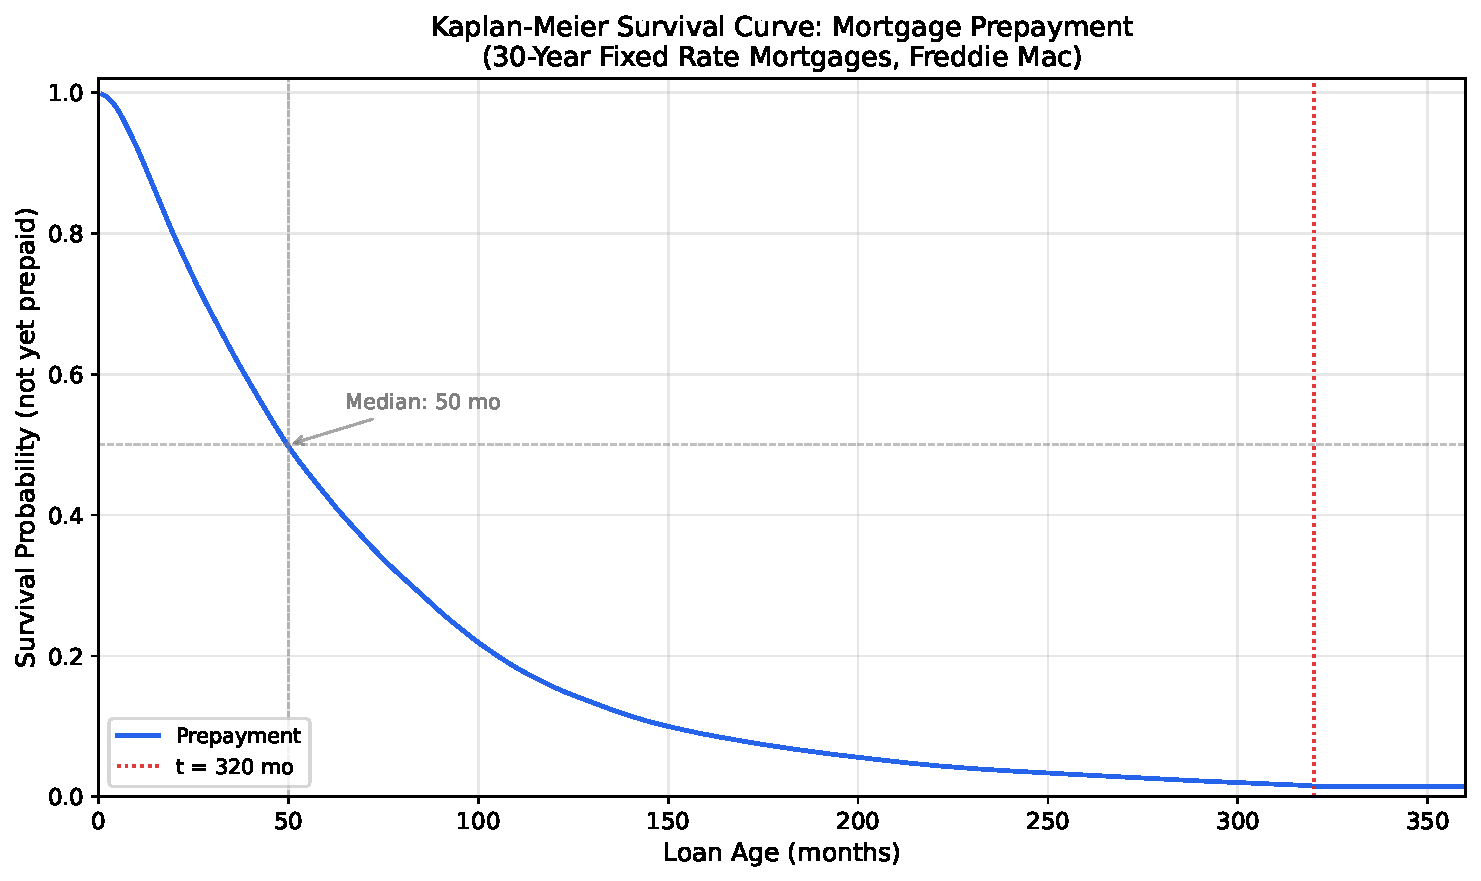
\includegraphics[width=0.6\textwidth]{figures/A_km_overall.pdf}
  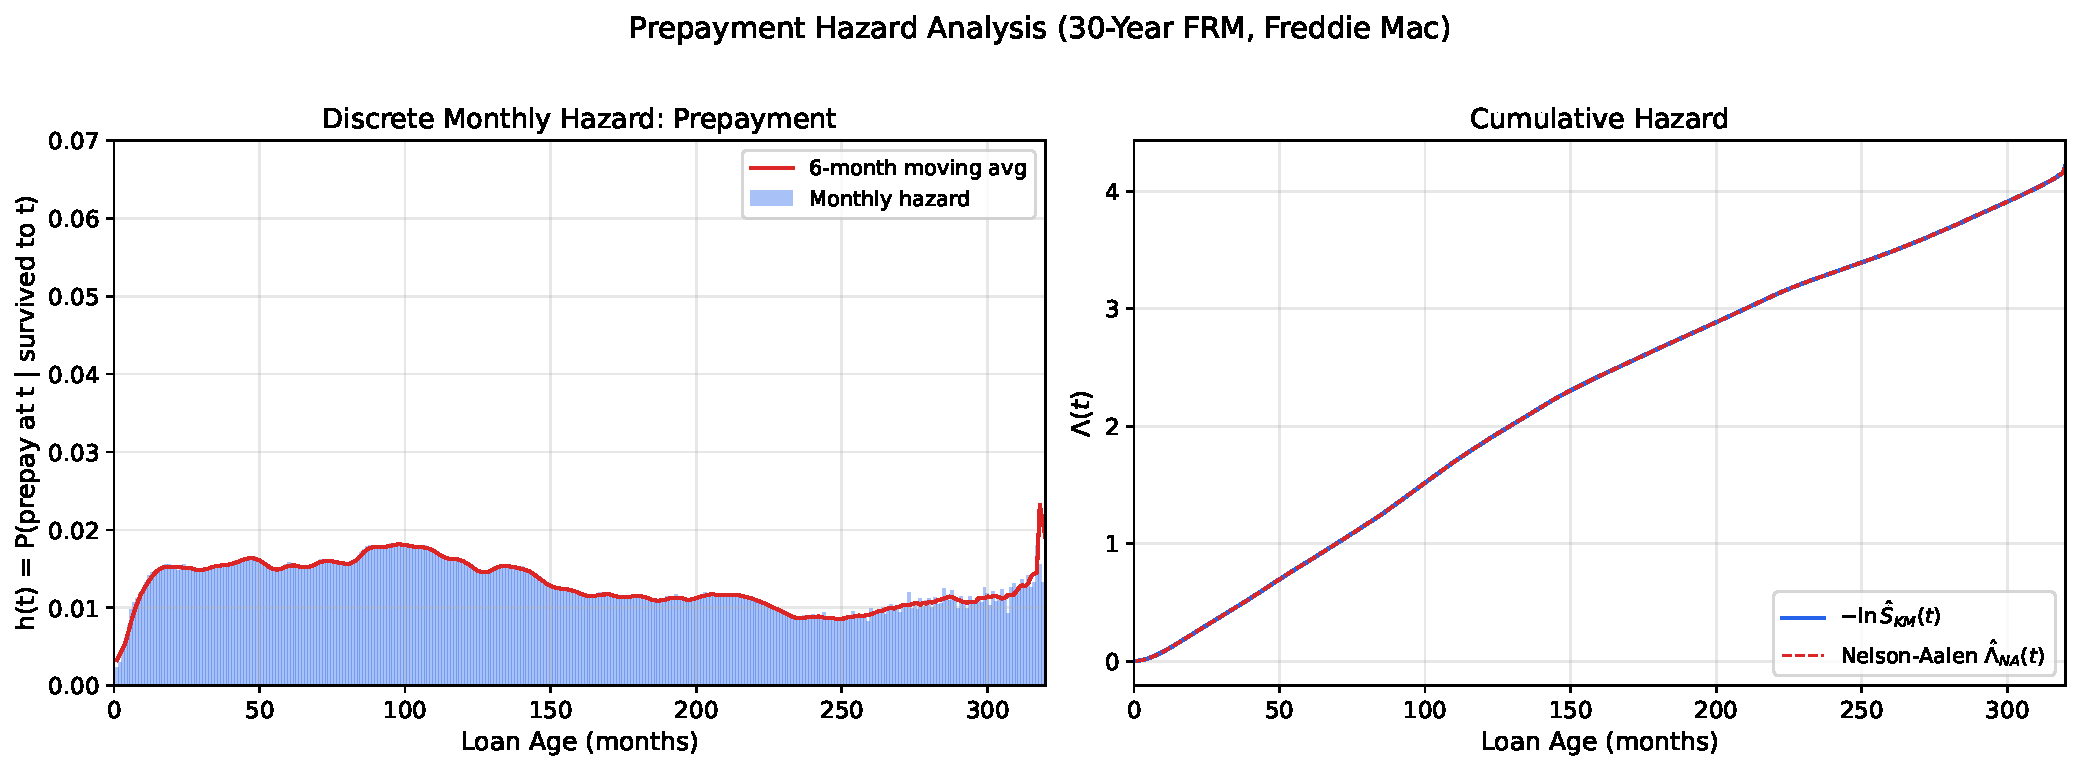
\includegraphics[width=0.9\textwidth]{figures/A_hazard_overall.pdf}
  \caption{\textbf{Part A.} KM survival curve on the full population (31.7M loans)}
\end{figure}

\textbf{Stratified curves.} The strongest single-variable effect is by \emph{vintage}: 1999--2003 loans prepay almost completely (96.3\%) with median 29 months, while 2020+ loans show only 16\% prepayment with median undefined (right-censored before reaching 50\%). LTV and FICO show modest, monotone gradients. Loan purpose is more nuanced --- no-cash-out refis prepay slightly more (70\%) than purchase loans (67\%) or cash-out refis (70\%), but with shifted timing.

\begin{figure}[h]
  \centering
  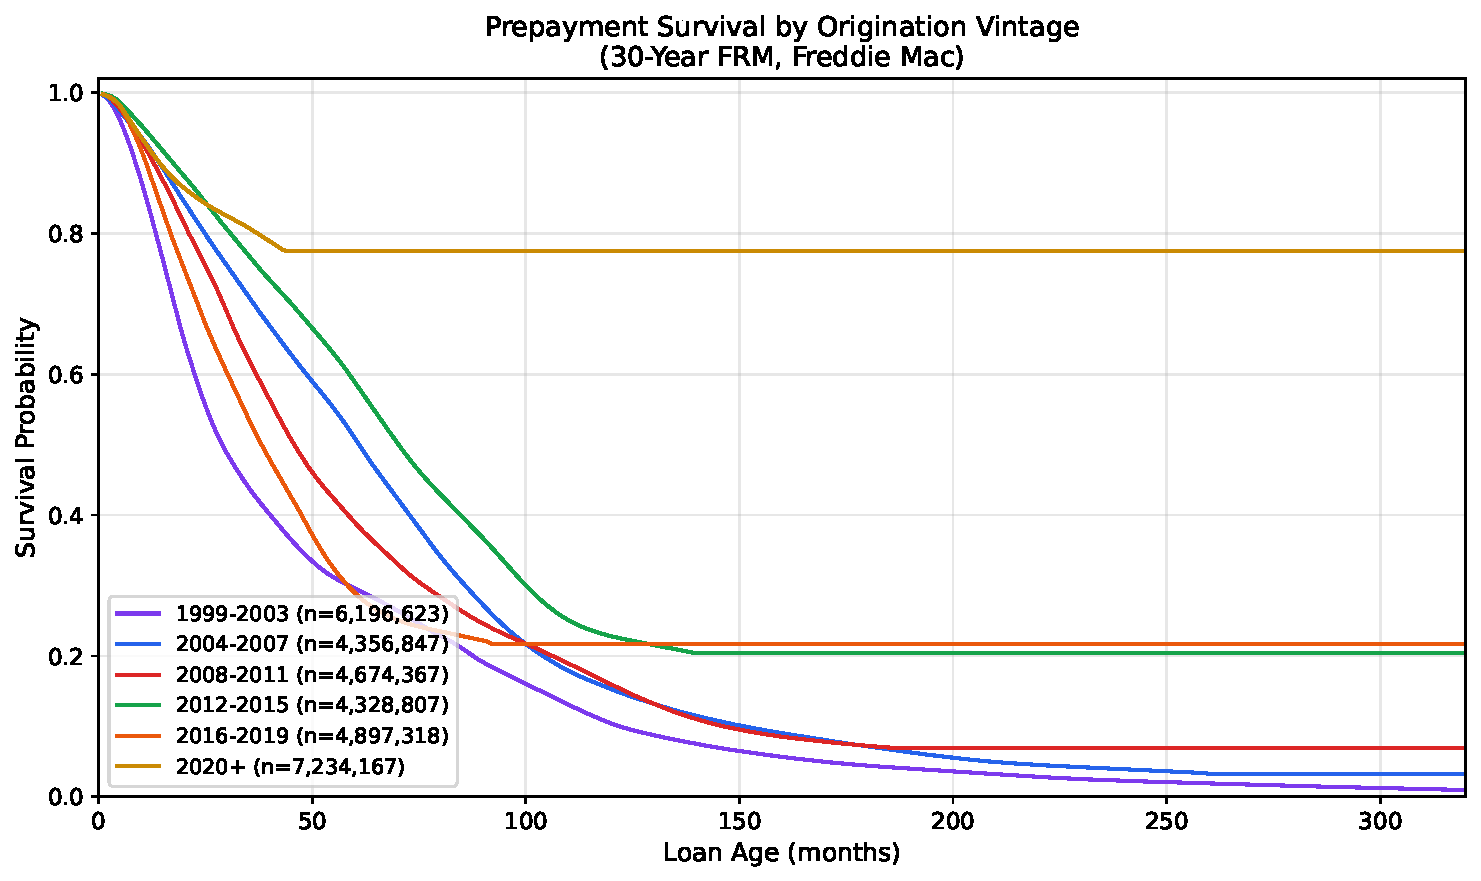
\includegraphics[width=0.49\textwidth]{figures/A_km_by_vintage.pdf}\hfill
  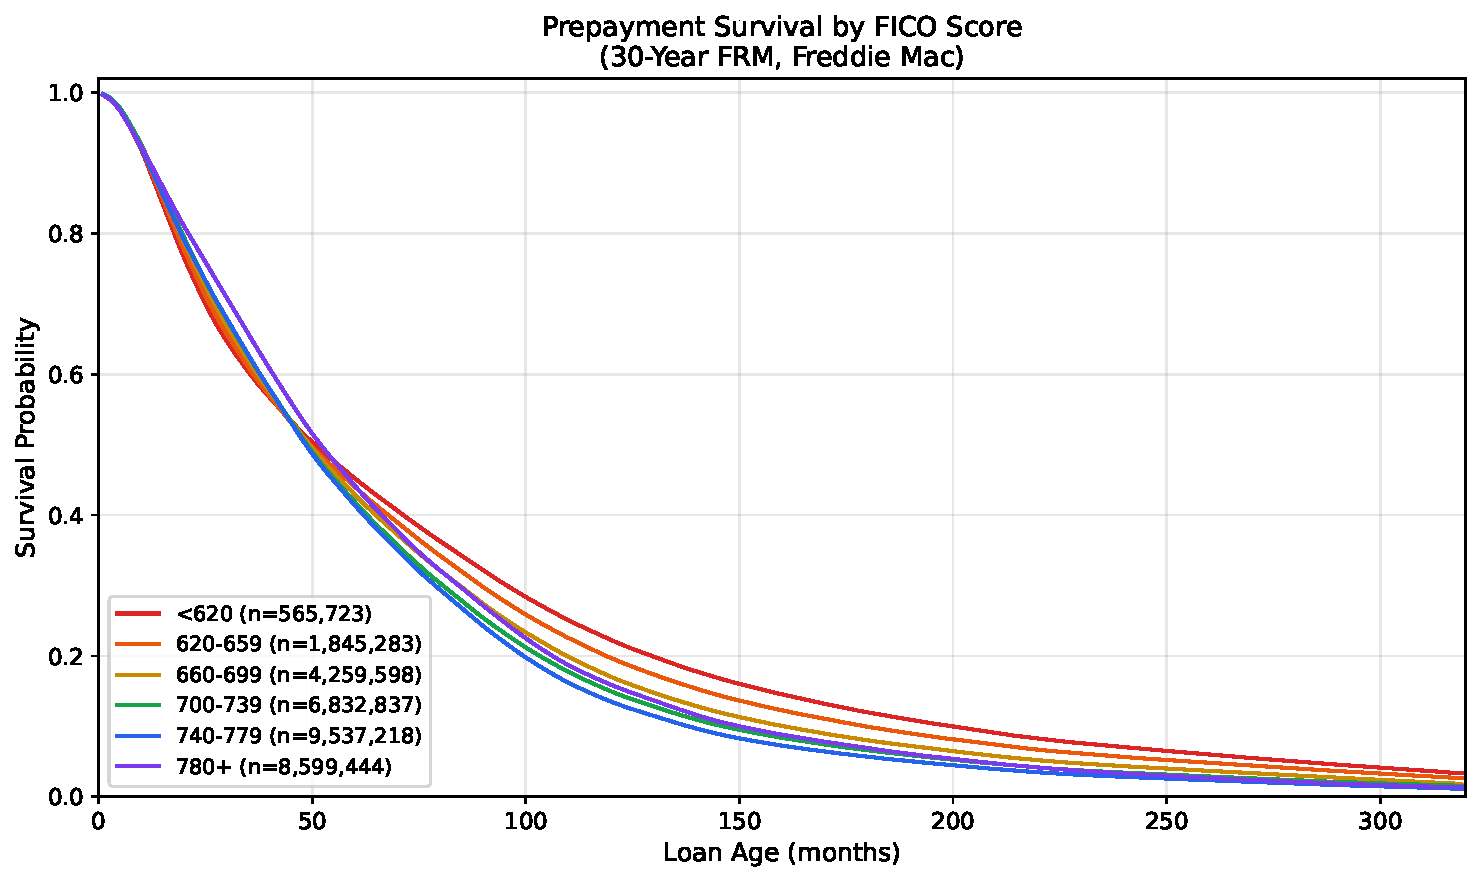
\includegraphics[width=0.49\textwidth]{figures/A_km_by_fico.pdf}
  \caption{\textbf{Part A stratification.} Left: by vintage cohort (rate environment dominates). Right: by FICO bucket (more modest, monotone gradient).}
\end{figure}

\begin{figure}[h]
  \centering
  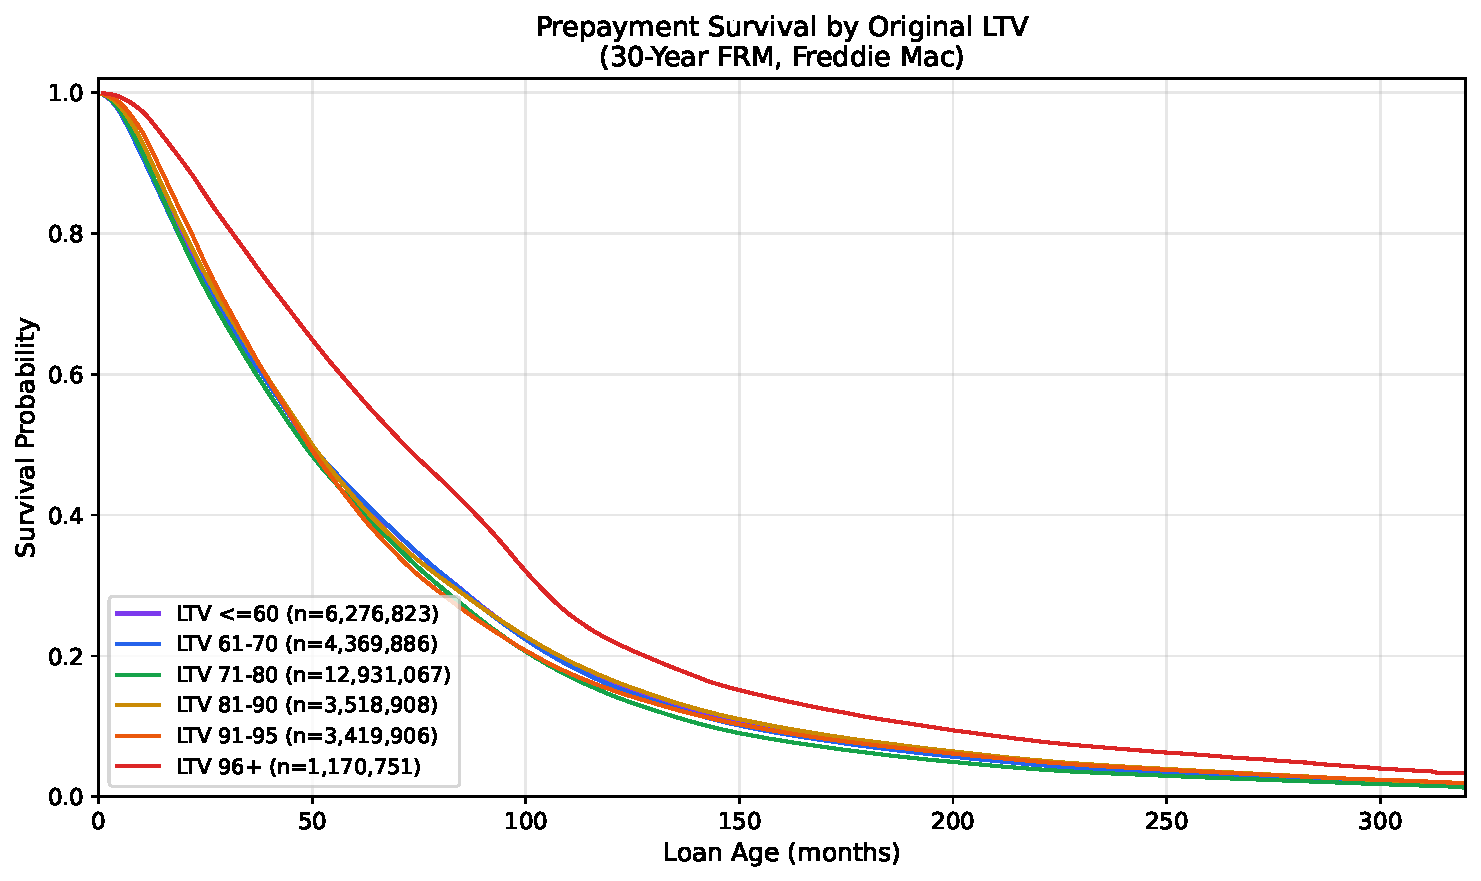
\includegraphics[width=0.49\textwidth]{figures/A_km_by_ltv.pdf}\hfill
  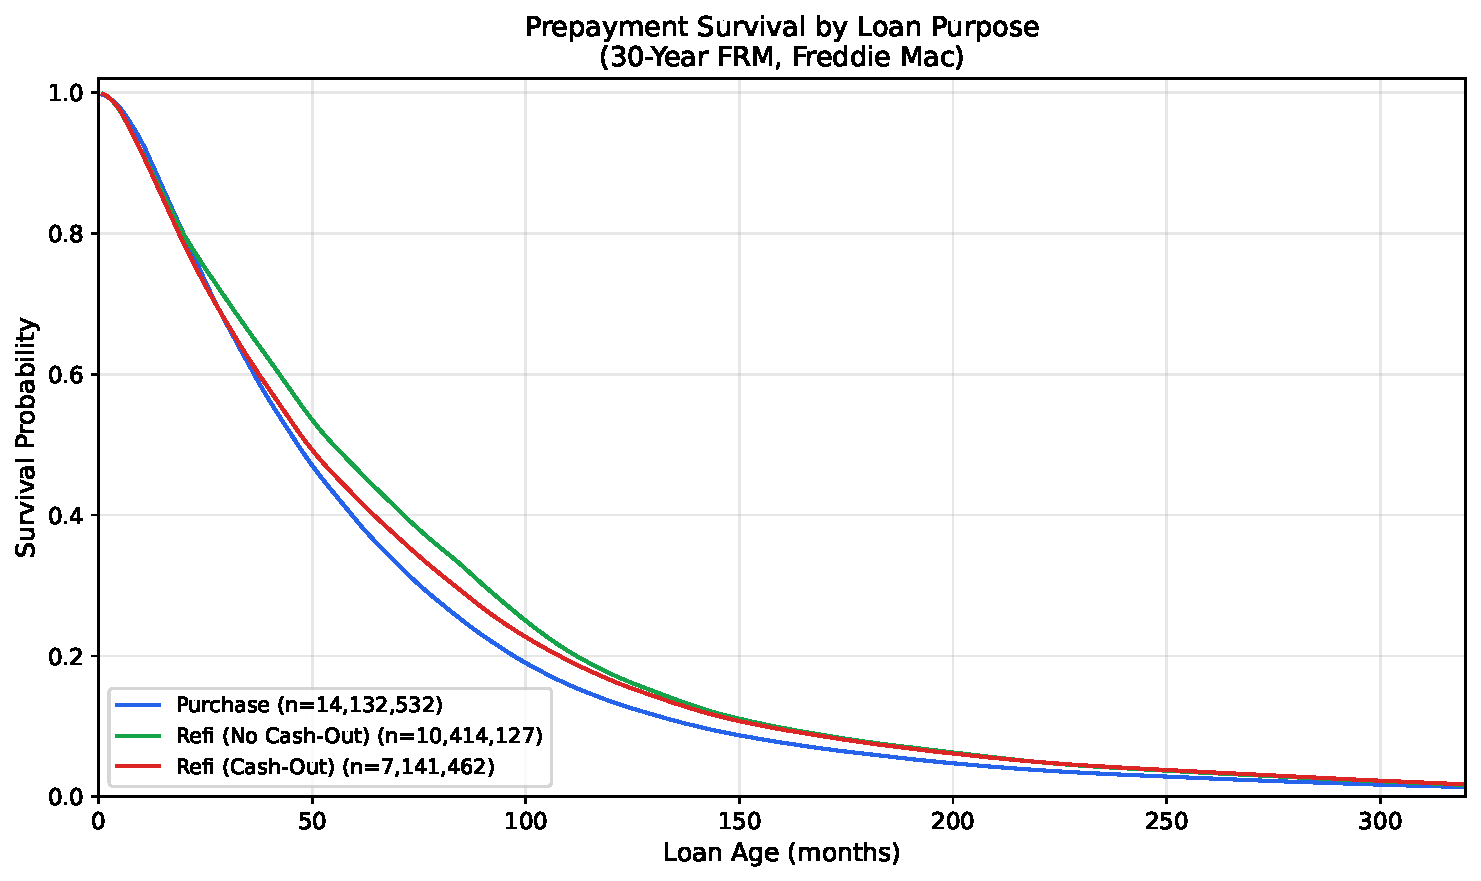
\includegraphics[width=0.49\textwidth]{figures/A_km_by_purpose.pdf}
  \caption{\textbf{Part A stratification, continued.} Left: by original LTV bucket. Right: by loan purpose. LTV separates less strongly than vintage, while loan-purpose curves show timing differences between purchase and refinance populations.}
\end{figure}

Vintage is the dominant driver as a proxy for origination-rate environment and the subsequent refinance opportunity. FICO and LTV show smaller monotone credit-quality gradients; loan purpose effects are non-monotone with timing differences between purchase and refinance populations.

% =================================================================
\section{Part B --- Cox Proportional Hazards}
% =================================================================

\textbf{Setup.} 5\% sample (1.58M loans, 1.08M events). 15 origination covariates (continuous standardized to z-scores; categorical as one-hot dummies with one reference). Fit via lifelines with $\ell_2$ penalizer 0.001.

\textbf{Base model.} Concordance index 0.6257 (modest; Cox is a one-parameter-per-covariate model on highly nonlinear data). The largest hazard ratios:
\begin{itemize}[leftmargin=1.2em,itemsep=2pt,topsep=2pt]
  \item \textbf{Original interest rate} (z): $\text{HR} = 1.58$ --- the dominant prepayment driver. Borrowers with high origination rates have the most refinancing incentive when rates fall.
  \item \textbf{Original UPB} (z): $\text{HR} = 1.29$ --- larger loans prepay more, consistent with refinancing fixed costs being amortized over larger principal.
  \item \textbf{Investment property}: $\text{HR} = 0.80$ --- investors prepay less (lower mobility, different tax treatment).
  \item \textbf{DTI missing}: $\text{HR} = 0.82$ --- DTI=999 is the Relief Refinance flag (FAQ Q67); these loans behave differently.
\end{itemize}

\textbf{Vintage-macro extension.} Adding four FRED macroeconomic series joined at origination (\texttt{FirstPaymentDate}) raises concordance to 0.6428 (improvement $\Delta C = +0.017$, $\Delta\text{AIC} = -28{,}510$):
\begin{itemize}[leftmargin=1.2em,itemsep=2pt,topsep=2pt]
  \item \textbf{10y Treasury rate at origination}: $\text{HR} = 0.78$ --- borrowers whose loans were originated when long rates were high subsequently prepay more (relative to those originated in low-rate environments), because they are more likely to encounter a rate-cut refinance opportunity.
  \item \textbf{HPI YoY at origination}: $\text{HR} = 0.89$ --- loans originated during housing booms prepay less than those originated in flat/declining markets.
  \item \textbf{Unemployment at origination}: $\text{HR} = 0.89$ --- consistent with the Sadhwani et al.\ 2021 ``labor market shock'' channel.
\end{itemize}

\textbf{Caveat.} These are vintage-macro covariates --- the macro state at the time of origination, \emph{not} time-varying through the loan's life. A truly dynamic Cox model with time-dependent covariates would require the full loan-month panel, which exceeds our memory budget.

\textbf{Proportional hazards diagnostic.} The Schoenfeld residual test rejects PH for 12 of 15 covariates at $\alpha = 0.05$. This is the standard finding on mortgage data and is the principal motivation for moving beyond Cox.

\begin{figure}[h]
  \centering
  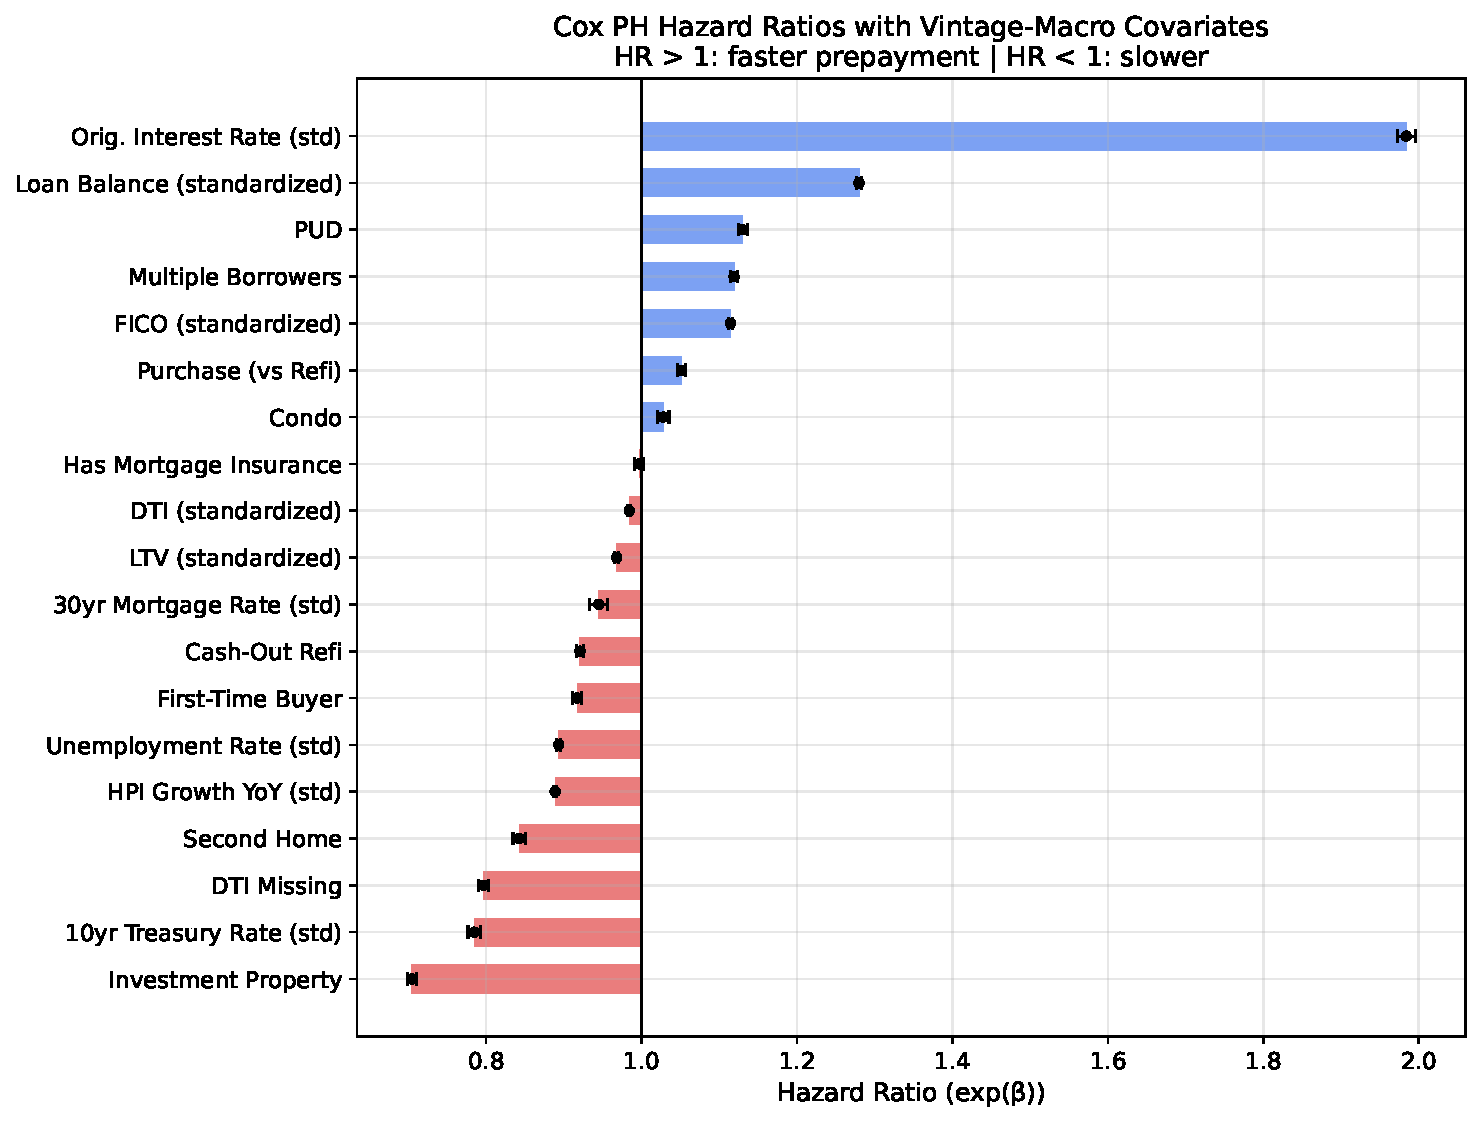
\includegraphics[width=0.49\textwidth]{figures/B_hazard_ratios_macro.pdf}\hfill
  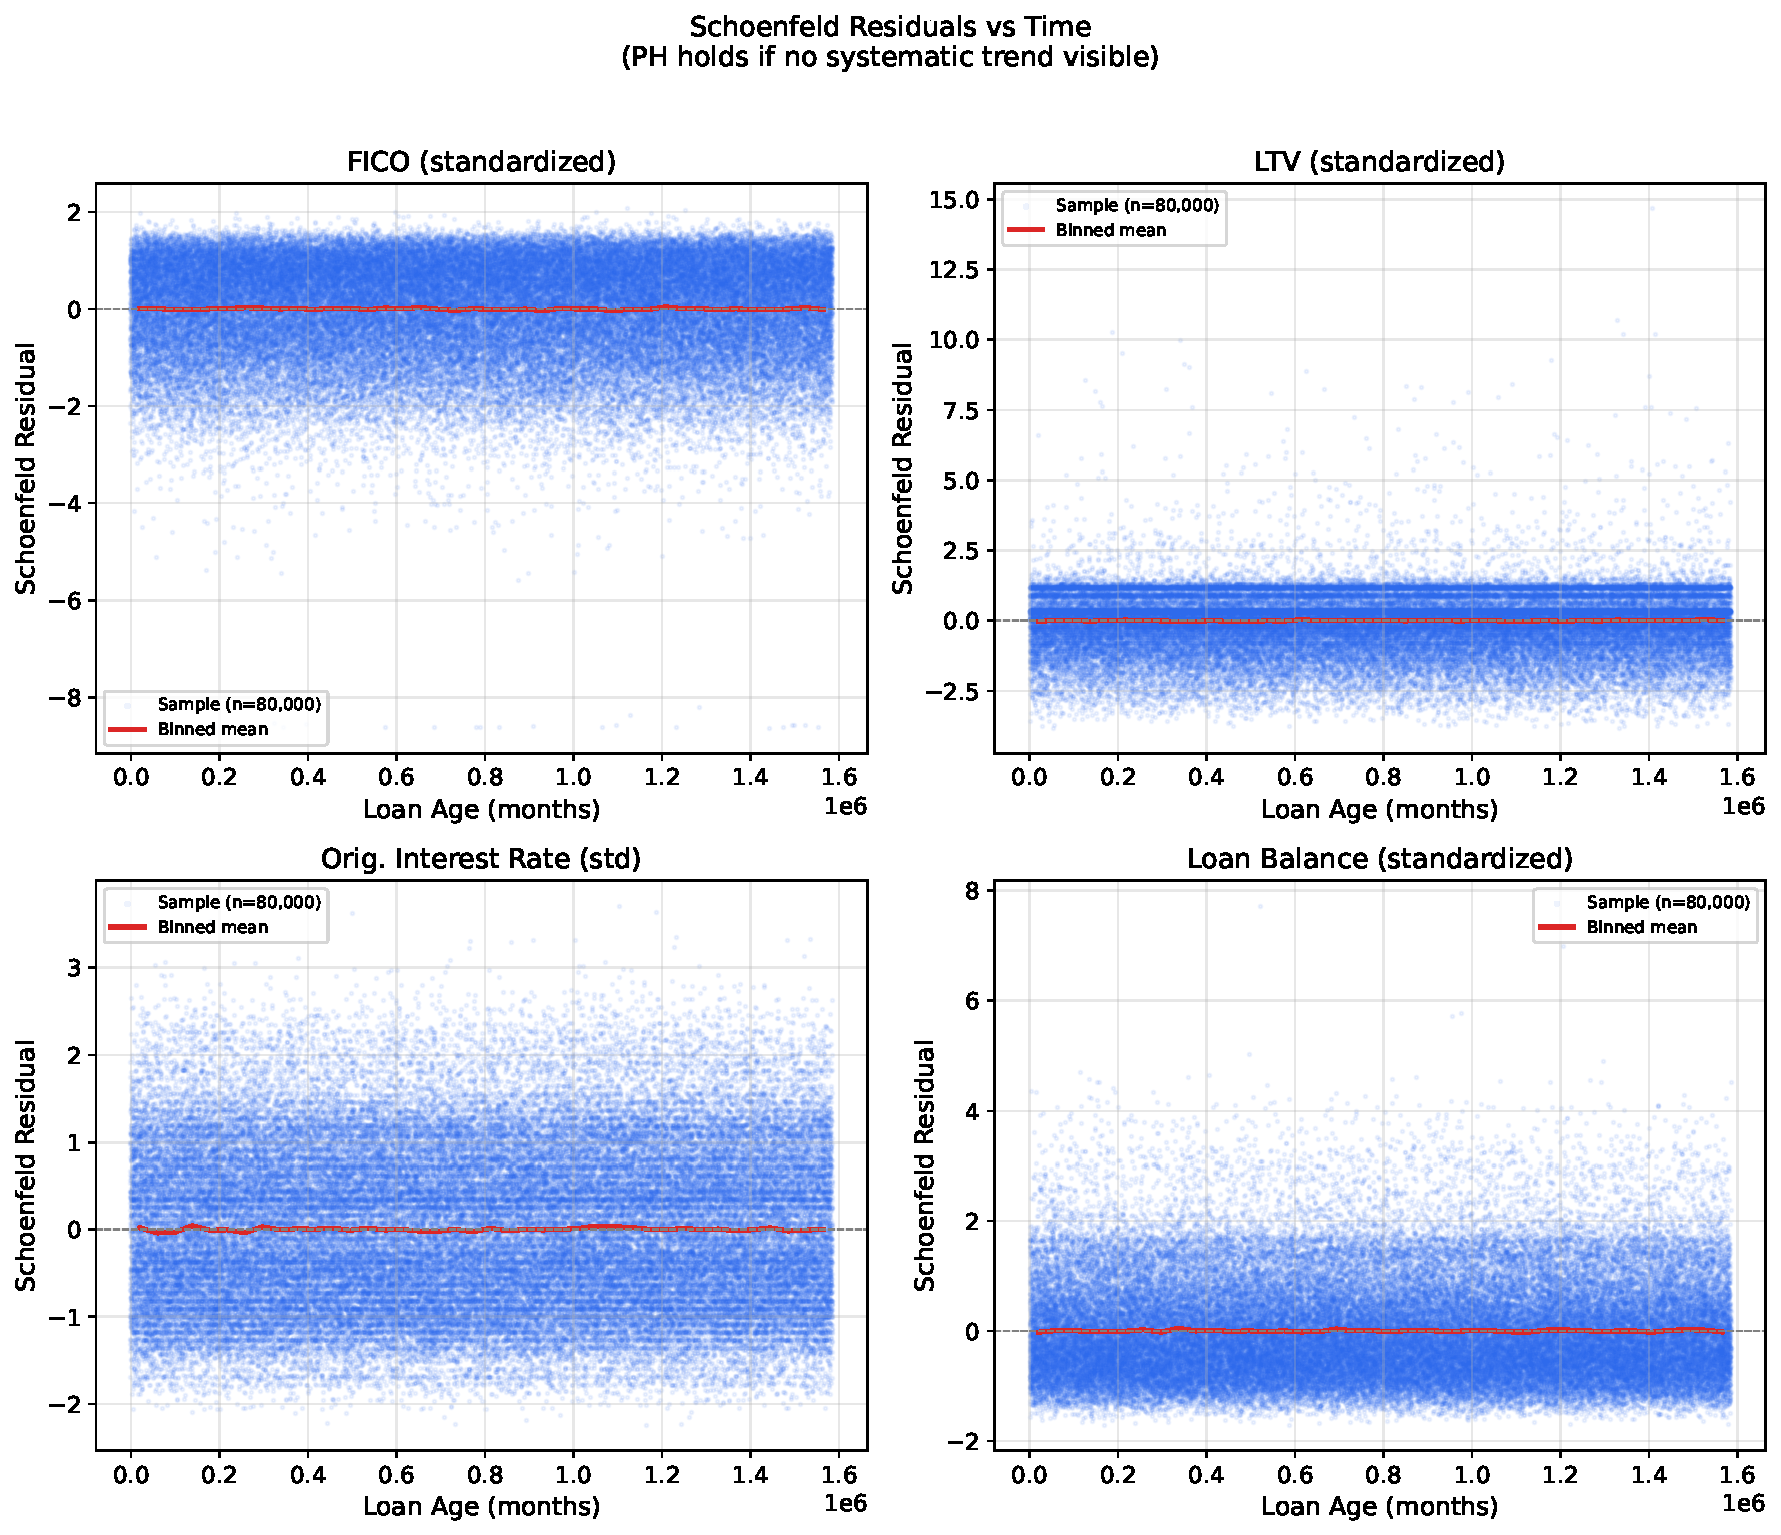
\includegraphics[width=0.49\textwidth]{figures/B_ph_test.pdf}
  \caption{\textbf{Part B.} Left: hazard ratios from the macro Cox model (HR$>$1 increases prepayment hazard). Right: Schoenfeld PH-test p-values --- 12/15 covariates show evidence of PH violation.}
\end{figure}

% =================================================================
\section{Part C --- Machine Learning Models}
% =================================================================

\textbf{Setup.} 10\% sample, 1.85M training and 597k test loans, 68 features post one-hot. We fit four models: Logistic Regression with $\ell_2$ regularization (using its own scaler internally), Random Forest (200 trees), LightGBM (early-stopping via held-out validation), and a Cox baseline using lifelines. Each model is fit per-horizon as a binary classifier targeting $\mathbf{1}\{\text{prepaid by } T\}$, with cause-specific exclusions as described.

\textbf{Out-of-sample AUC.}

\begin{center}
  \small
  \begin{tabular}{lcccc}
    \toprule
    Model         & T=12   & T=24   & T=36   & T=60   \\
    \midrule
    Cox           & 0.6635 & 0.6571 & 0.6596 & 0.6650 \\
    Random Forest & 0.6706 & 0.6519 & 0.6718 & 0.6803 \\
    LightGBM      & 0.6805 & 0.6738 & 0.6899 & 0.6825 \\
    LogReg        & 0.6908 & 0.6670 & 0.6837 & 0.7043 \\
    \bottomrule
  \end{tabular}
\end{center}

The four models cluster in the 0.65--0.70 AUC band. Logistic regression is competitive --- in fact best at $T{=}12$ and $T{=}60$ --- which suggests that the marginal effects in the data are largely linear-additive in z-scored covariates and that tree models' axis-aligned splits don't unlock much extra signal at these horizons. LightGBM has the best Brier scores and is consistently top-2.

\textbf{Calibration.} All four models are reasonably well-calibrated, with LightGBM and LogReg showing the tightest fit to the diagonal. Cox is slightly under-confident at the high end (the linear-predictor model can't push probabilities very close to 1 even when warranted).

\textbf{Top-decile lift.} For an investor interested in identifying loans most likely to prepay, the lift in the top decile is most informative at moderate horizons: at $T{=}12$, the top decile contains 27.6\% prepayments (LightGBM) versus a 10.75\% base rate, for a lift of 2.57$\times$. Logistic regression achieves nearly identical lift (2.54$\times$). The lift saturates at long horizons because the base prepayment rate exceeds 70\% at $T{=}60$ --- there is simply not much room in the top decile for additional concentration.

\begin{figure}[h]
  \centering
  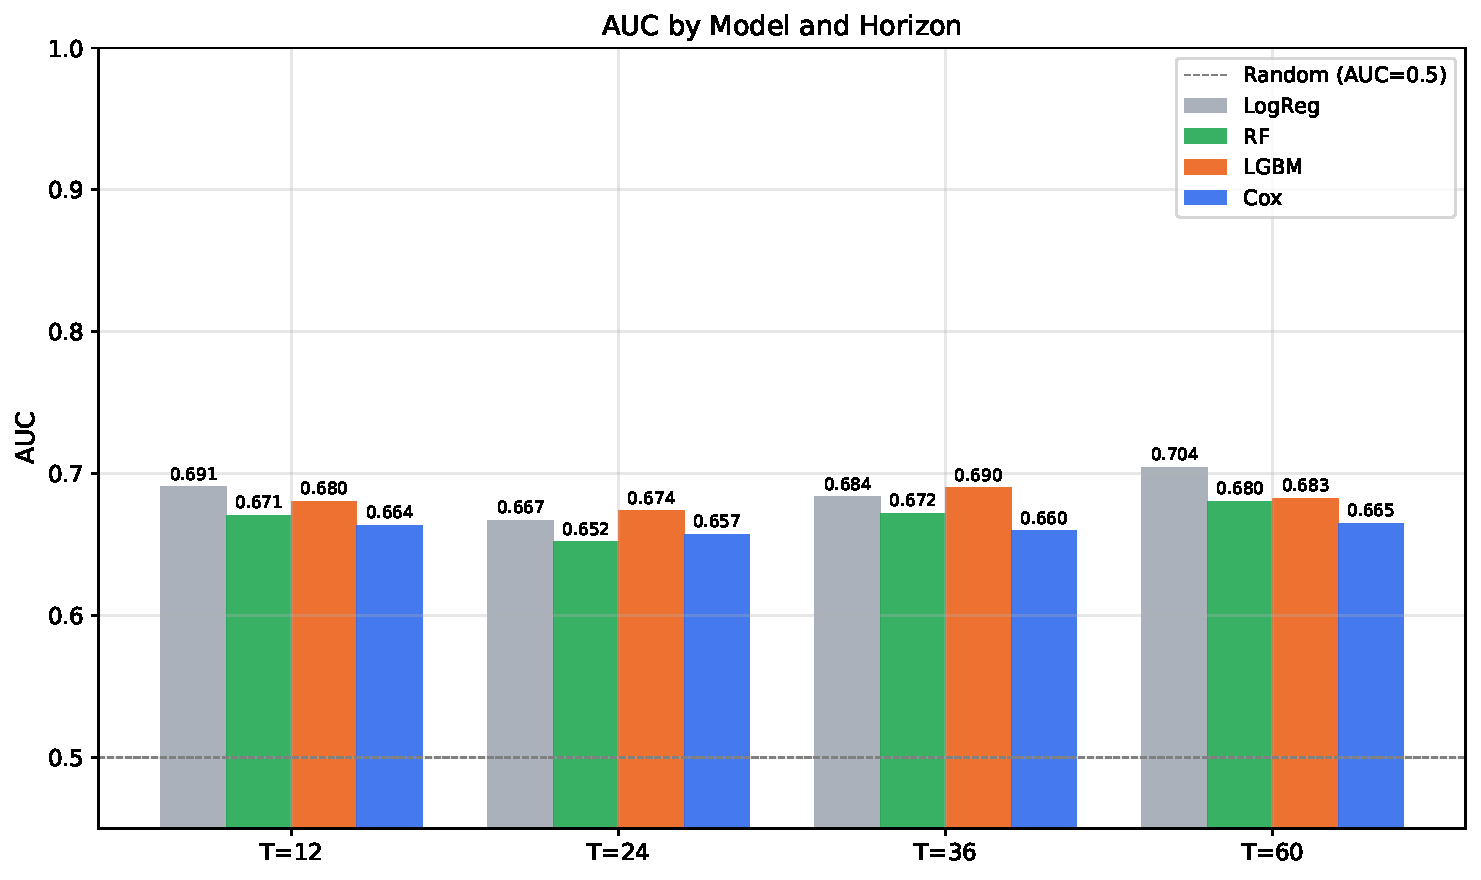
\includegraphics[width=0.49\textwidth]{figures/C_auc_by_horizon.pdf}\hfill
  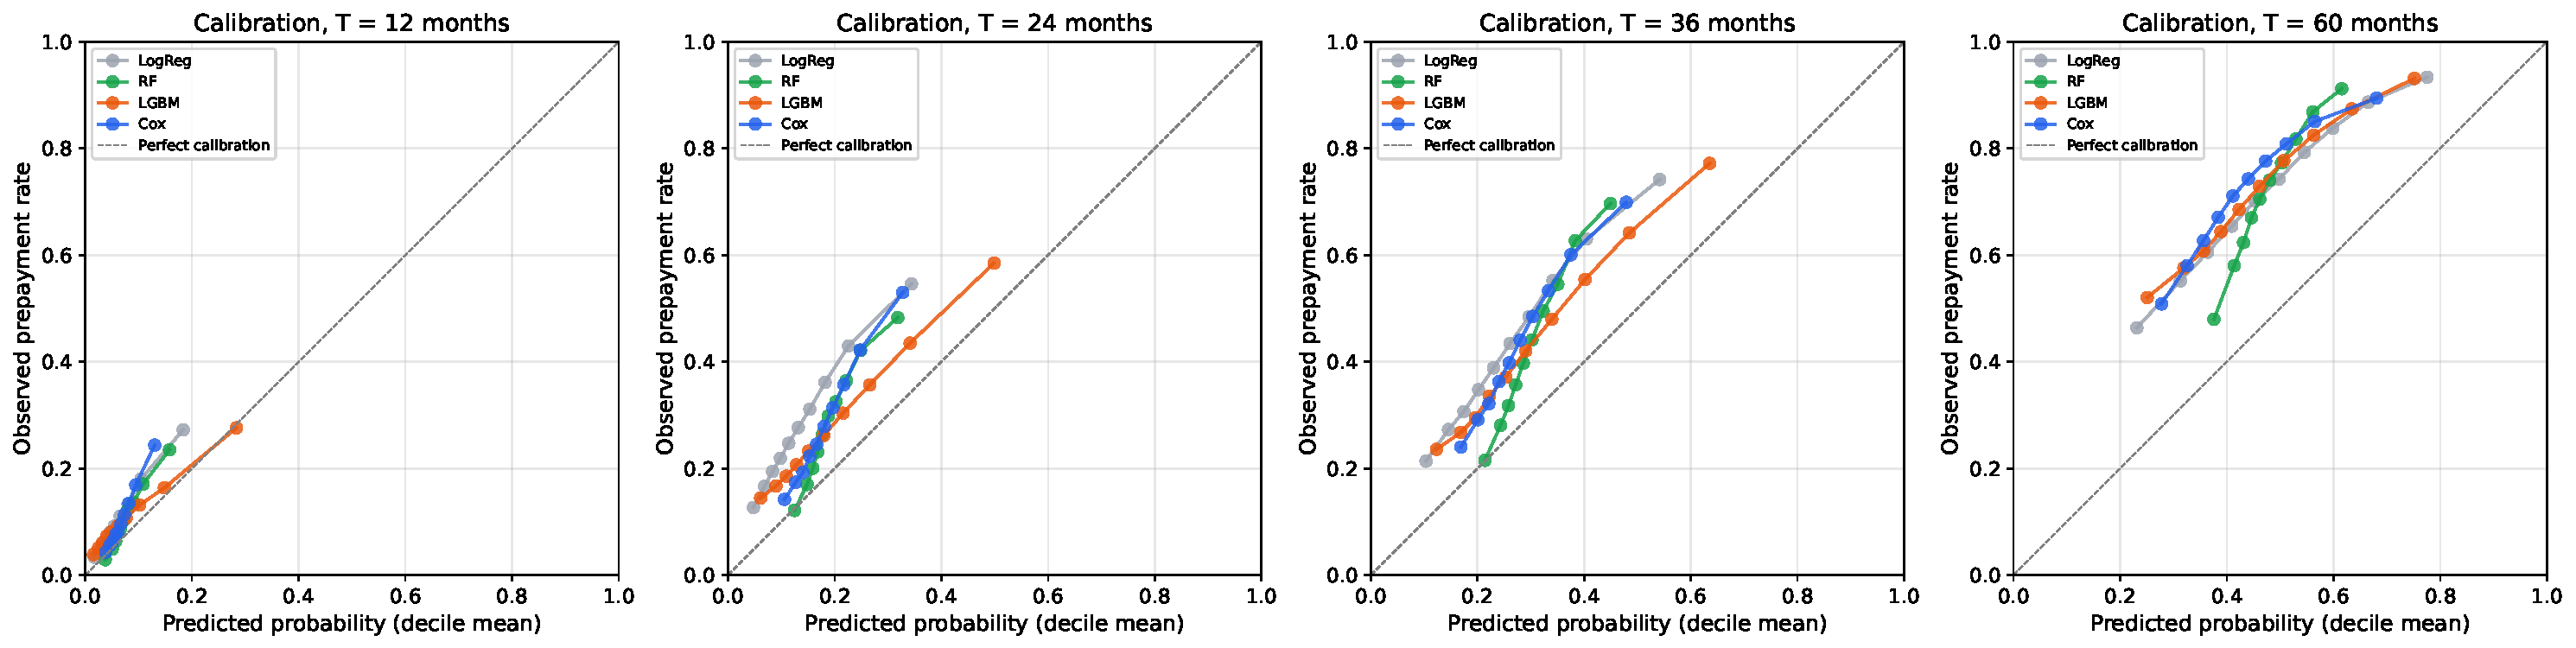
\includegraphics[width=0.49\textwidth]{figures/C_calibration.pdf}
  \caption{\textbf{Part C.} Left: AUC by model and horizon. Right: decile calibration plot.}
\end{figure}

\begin{figure}[h]
  \centering
  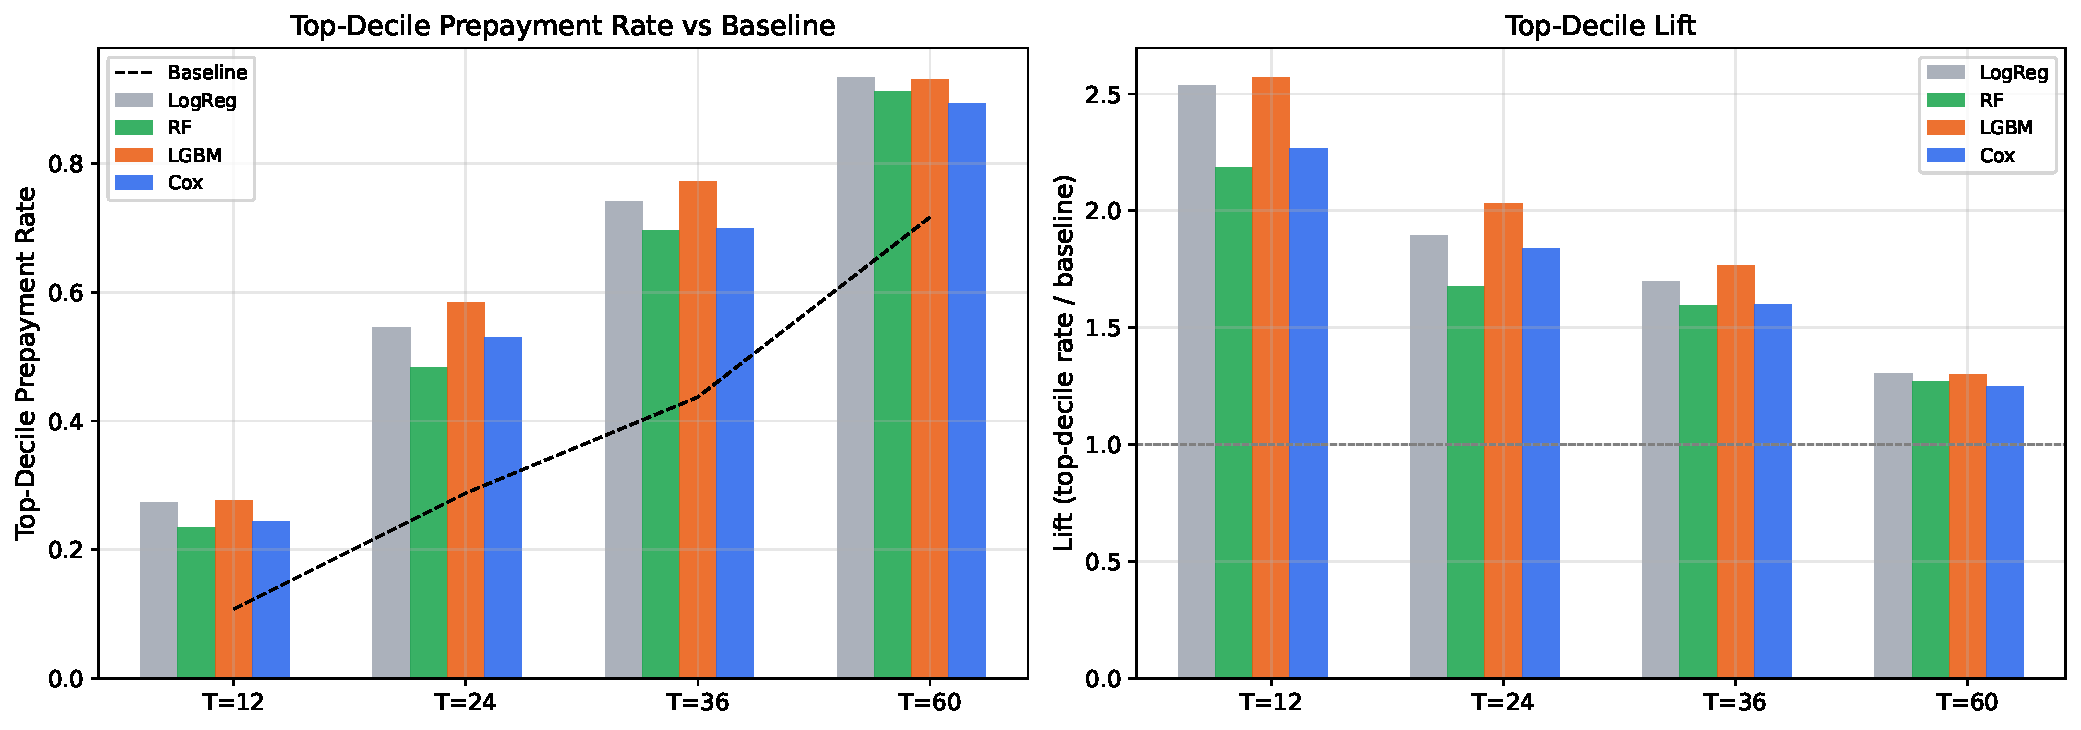
\includegraphics[width=0.65\textwidth]{figures/C_top_decile_lift.pdf}
  \caption{\textbf{Part C: top-decile lift.} Practical-investor metric --- among the top 10\% of test loans ranked by predicted prepay probability, what fraction actually prepays within horizon $T$, divided by the population base rate. Saturation at $T{=}60$ reflects the high base rate (71.7\%).}
\end{figure}

% =================================================================
\section{Part D --- Deep Cox Model}
% =================================================================

\textbf{Architecture.} 3 hidden layers $\times$ 64 ReLU units, batch normalization, dropout 0.1, no output bias (standard DeepSurv setup). 13{,}184 parameters versus 68 for the linear baseline.

\textbf{Training.} pycox's \texttt{CoxPH} with Adam ($\eta = 10^{-3}$), batch 512, max 50 epochs, early-stopping patience 8 on validation partial-likelihood loss. The Cox partial likelihood is computed per minibatch (risk sets are batch-local --- the standard pycox / DeepSurv stochastic approximation). Total CPU runtime: 17 minutes for Deep, 1 minute for Linear baseline. Breslow baseline hazards estimated post-fit on the full training set.

\textbf{D(v) ablation --- Linear vs Deep.} The linear baseline uses the identical pycox infrastructure with \texttt{num\_nodes=[]}, so it is functionally a SGD-fit classical Cox. This is the cleanest possible isolation of the nonlinearity contribution: same data, same optimizer, same baseline-hazard estimator.

\begin{center}
  \small
  \begin{tabular}{lcccc}
    \toprule
    Horizon & Linear AUC & Deep AUC & $\Delta$AUC & $\Delta$LogLoss \\
    \midrule
    12      & 0.6807     & 0.6837   & $+0.0030$   & $-0.0050$       \\
    24      & 0.6738     & 0.7007   & $+0.0269$   & $-0.0267$       \\
    36      & 0.6772     & 0.7211   & $+0.0439$   & $-0.0517$       \\
    60      & 0.6848     & 0.7292   & $+0.0445$   & $-0.1020$       \\
    \bottomrule
  \end{tabular}
\end{center}

The gap widens monotonically with horizon. The interpretation is clean: at $T{=}12$, the prepayment decision is largely driven by linear effects (rate differential, FICO, balance); but as horizon extends, \emph{interaction} effects between borrower characteristics and the macro/temporal environment become increasingly important, and these are exactly what the network captures.

\textbf{D(iv) head-to-head.} Combined comparison with all Part C models:

\begin{center}
  \small
  \begin{tabular}{lcccc}
    \toprule
    Model                   & T=12            & T=24            & T=36            & T=60            \\
    \midrule
    Cox                     & 0.6635          & 0.6571          & 0.6596          & 0.6650          \\
    Random Forest           & 0.6706          & 0.6519          & 0.6718          & 0.6803          \\
    LightGBM                & 0.6805          & 0.6738          & 0.6899          & 0.6825          \\
    LinearCox (D, ablation) & 0.6807          & 0.6738          & 0.6772          & 0.6848          \\
    LogReg                  & 0.6908          & 0.6670          & 0.6837          & 0.7043          \\
    \textbf{DeepCox}        & \textbf{0.6837} & \textbf{0.7007} & \textbf{0.7211} & \textbf{0.7292} \\
    \bottomrule
  \end{tabular}
\end{center}

DeepCox is best at every horizon $\geq 24$ months, often by 0.04--0.05 AUC --- a substantial margin in this domain. At $T{=}12$ LogReg edges it slightly. We also note that LinearCox $>$ Cox at every horizon (by $\sim$0.015--0.020); this is consistent --- both are linear-predictor + Breslow baseline, but LinearCox uses Part C's full encoded feature matrix while the lifelines-fit Cox uses the more parsimonious Part B specification.

\begin{figure}[h]
  \centering
  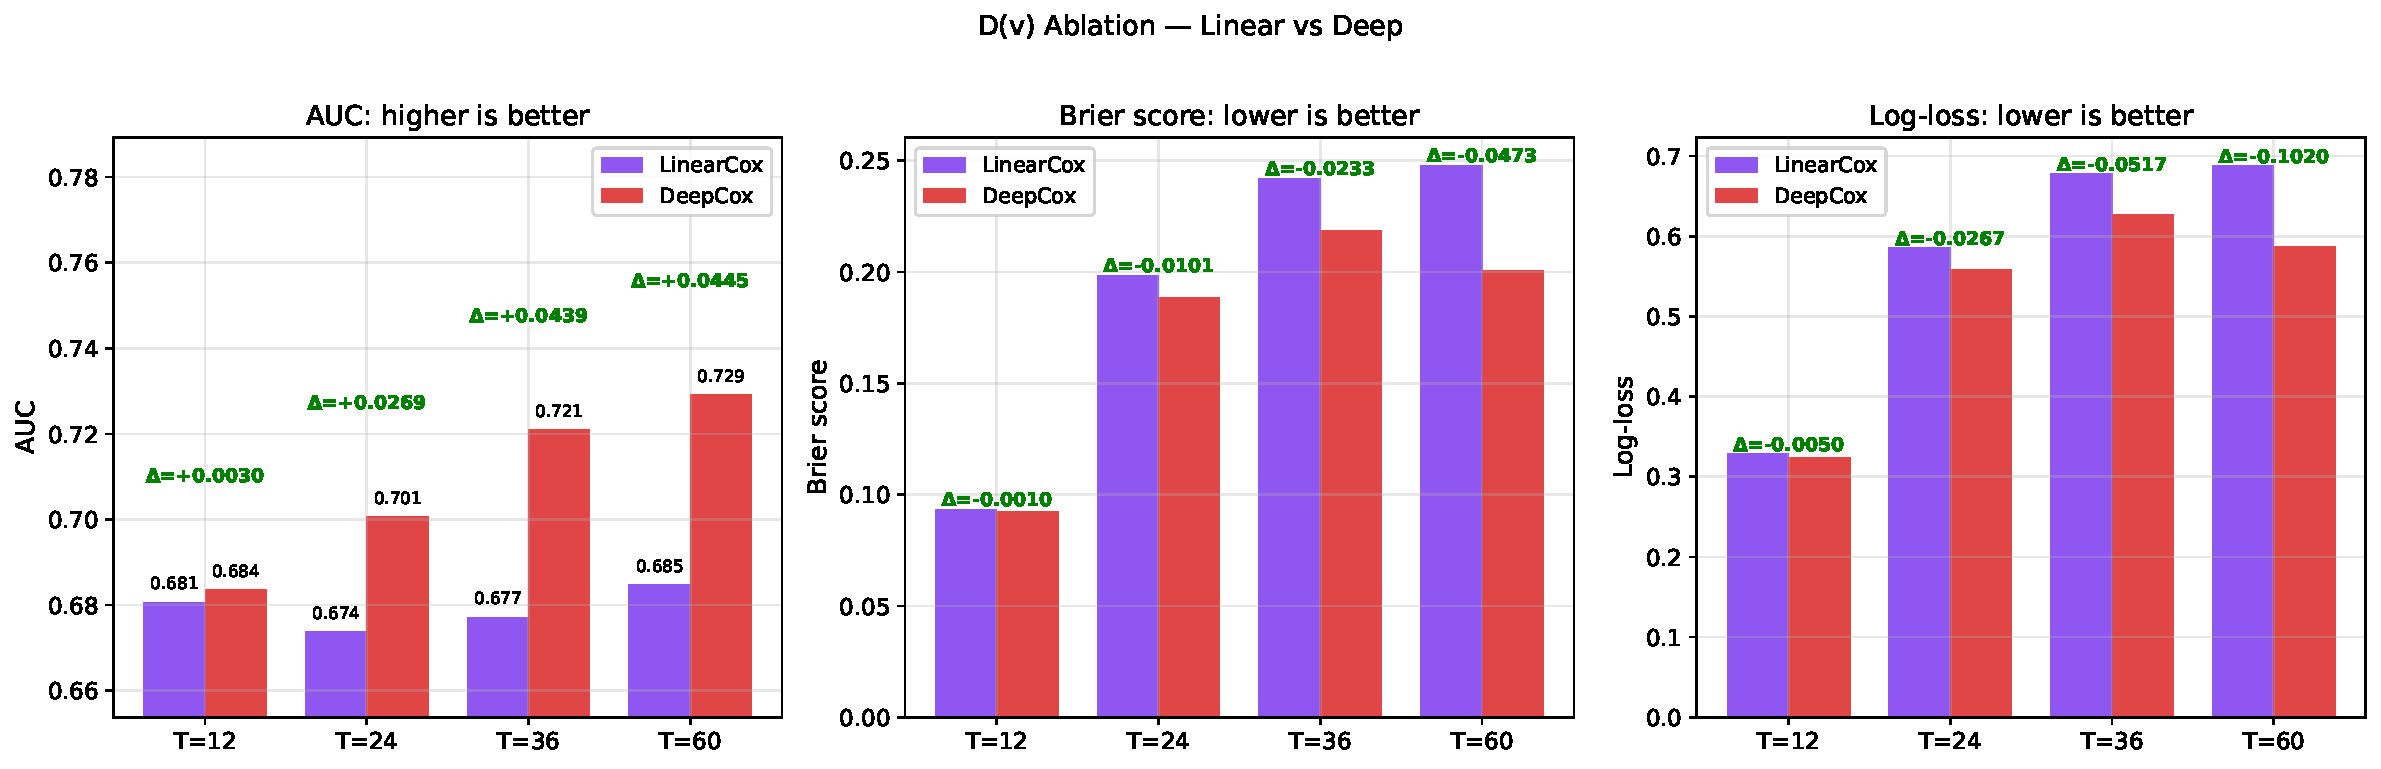
\includegraphics[width=0.48\textwidth]{figures/D_ablation_bars.pdf}\hfill
  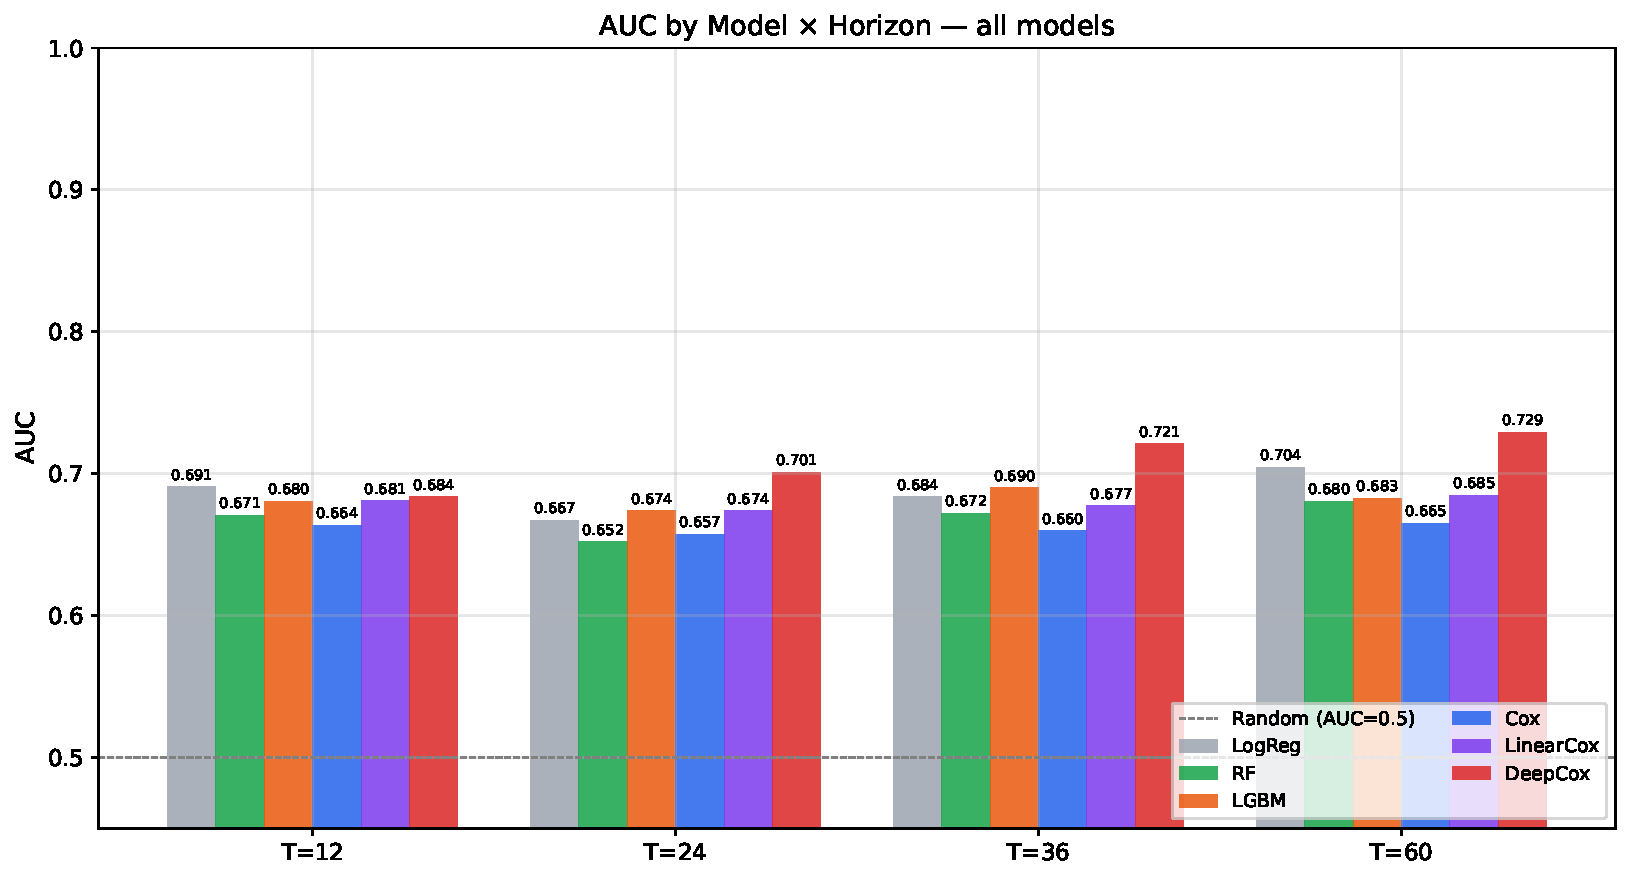
\includegraphics[width=0.48\textwidth]{figures/D_auc_by_horizon.pdf}
  \caption{\textbf{Part D.} Left: D(v) Linear-vs-Deep ablation; Deep gain widens with horizon. Right: head-to-head AUC comparing all six models, with DeepCox winning at long horizons.}
\end{figure}

\textbf{Calibration and top-decile lift.} DeepCox is also the best-calibrated model at long horizons (predicted probabilities track the empirical prepayment rate close to the diagonal in the decile reliability plot). At moderate horizons ($T{=}24$, $T{=}36$) DeepCox also delivers the best top-decile lift among all six models: 2.08$\times$ at $T{=}24$ versus LightGBM's 2.03$\times$ and LogReg's 1.90$\times$. The combination of best AUC, best calibration, and best top-decile lift across long horizons makes DeepCox the dominant model in this study.

\begin{figure}[h]
  \centering
  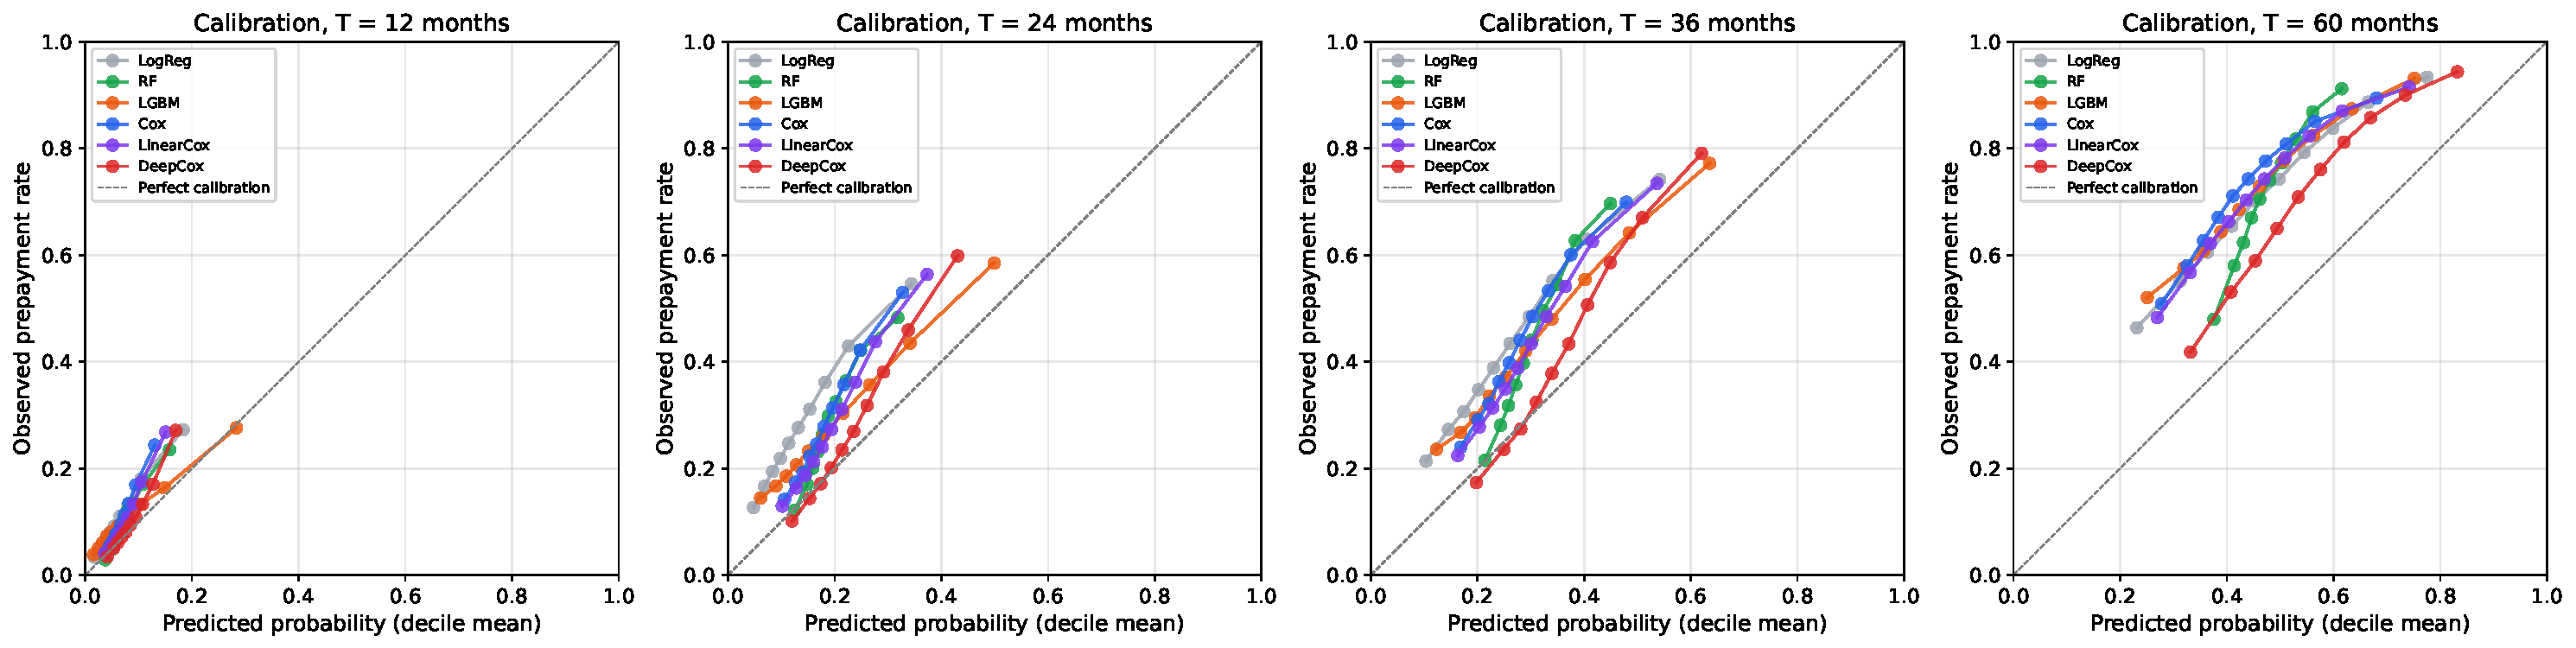
\includegraphics[width=0.49\textwidth]{figures/D_calibration.pdf}\hfill
  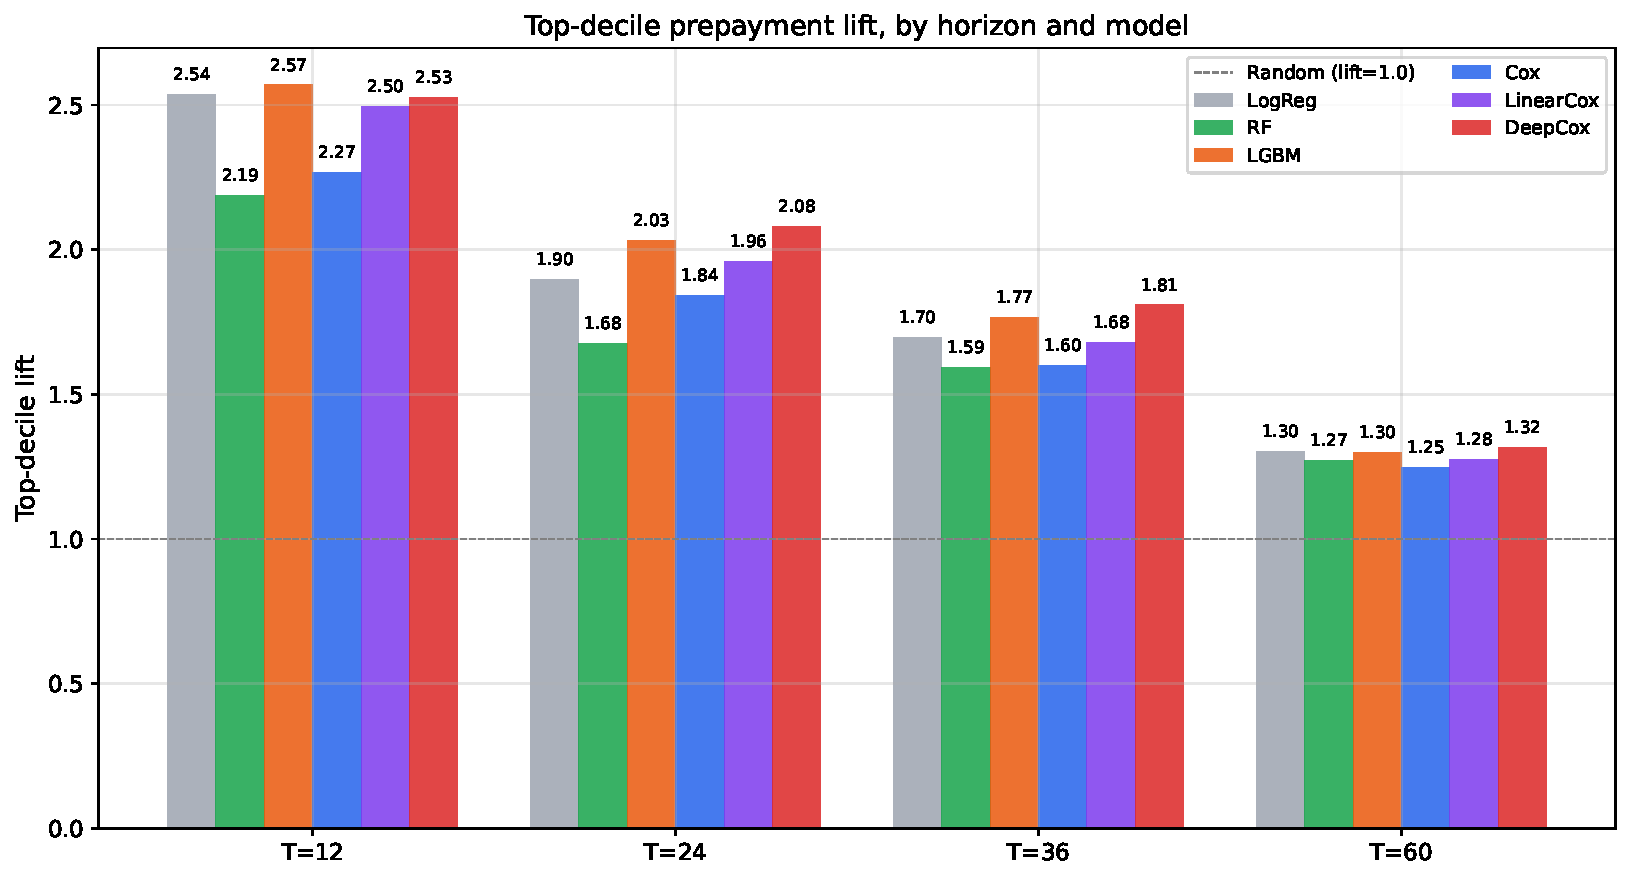
\includegraphics[width=0.49\textwidth]{figures/D_top_decile_lift.pdf}
  \caption{\textbf{Part D supporting plots.} Left: decile calibration for DeepCox vs LinearCox at all horizons. Right: top-decile lift comparison across all six models.}
\end{figure}

% =================================================================
\section{Part E --- Competing Risks, Time-Varying Cox, Neural Survival, and Scenario Analysis}
% =================================================================

Part E extends the prepayment-only framing of Parts A--D in four directions: explicit competing-risks modeling, time-varying covariates, a sequence-based neural survival model, and interest-rate scenario analysis translated into MBS cash flows.

% -----------------------------------------------------------------
\subsection{Part E(i) --- Competing Risks: Kaplan--Meier vs.\ Aalen--Johansen}

Prepayment and default are competing risks: each loan exits via exactly one cause, and treating one as random censoring distorts the other. The Aalen--Johansen (AJ) estimator keeps all exits in the risk-set denominator and provides a coherent probability partition, whereas the cause-specific Kaplan--Meier estimator used in Parts A--D censors competing exits and inflates the cause-specific incidence:
\[
  \hat{F}^{(k)}_{\mathrm{KM}}(t) = 1 - \prod_{t_j \le t}\!\left(1 - \frac{d_{j}^{(k)}}{n_j^{\mathrm{KM}}}\right),
  \qquad
  \hat{F}_k^{\mathrm{AJ}}(t) = \sum_{t_j \le t} \hat{S}(t_j^{-}) \cdot \frac{d_{kj}}{n_j}.
\]
AJ guarantees $\hat{F}^{(\mathrm{pre})}(t) + \hat{F}^{(\mathrm{def})}(t) + \hat{S}(t) = 1$ at every $t$; KM does not.

\textbf{Empirical bias.} Over the 1999--2025 Freddie Mac sample, KM overstates the prepayment CIF monotonically with horizon:

\begin{center}
  \small
  \begin{tabular}{lccc}
    \toprule
    Horizon & $\hat{F}_{\mathrm{KM}}$ & $\hat{F}_{\mathrm{AJ}}$ & Bias       \\
    \midrule
    5 yr    & 61.9\%                  & 61.4\%                  & $+$0.45 pp \\
    10 yr   & 84.6\%                  & 83.3\%                  & $+$1.31 pp \\
    20 yr   & 93.4\%                  & 91.8\%                  & $+$2.23 pp \\
    \bottomrule
  \end{tabular}
\end{center}

\begin{figure}[h]
  \centering
  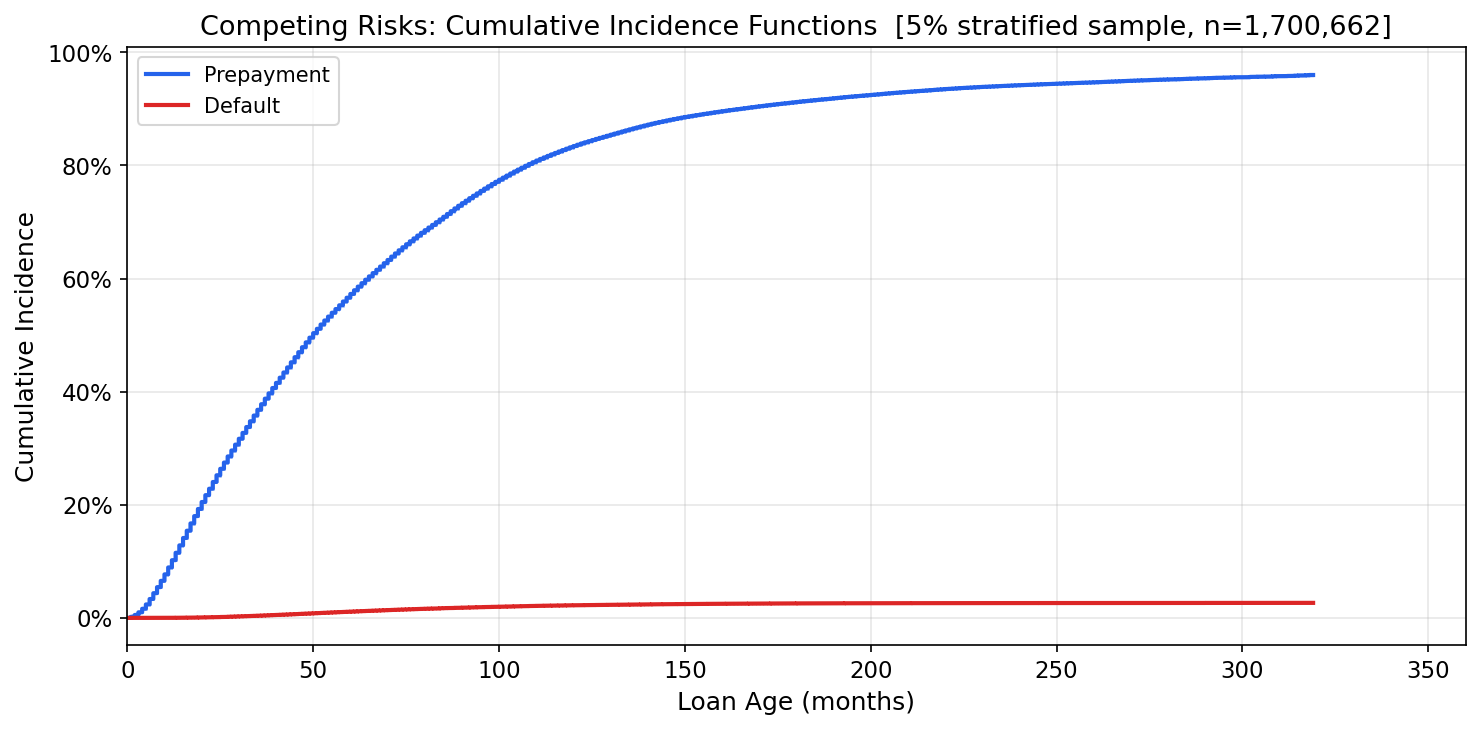
\includegraphics[width=0.55\textwidth]{E1_competing_risks_cif.png}\hfill
  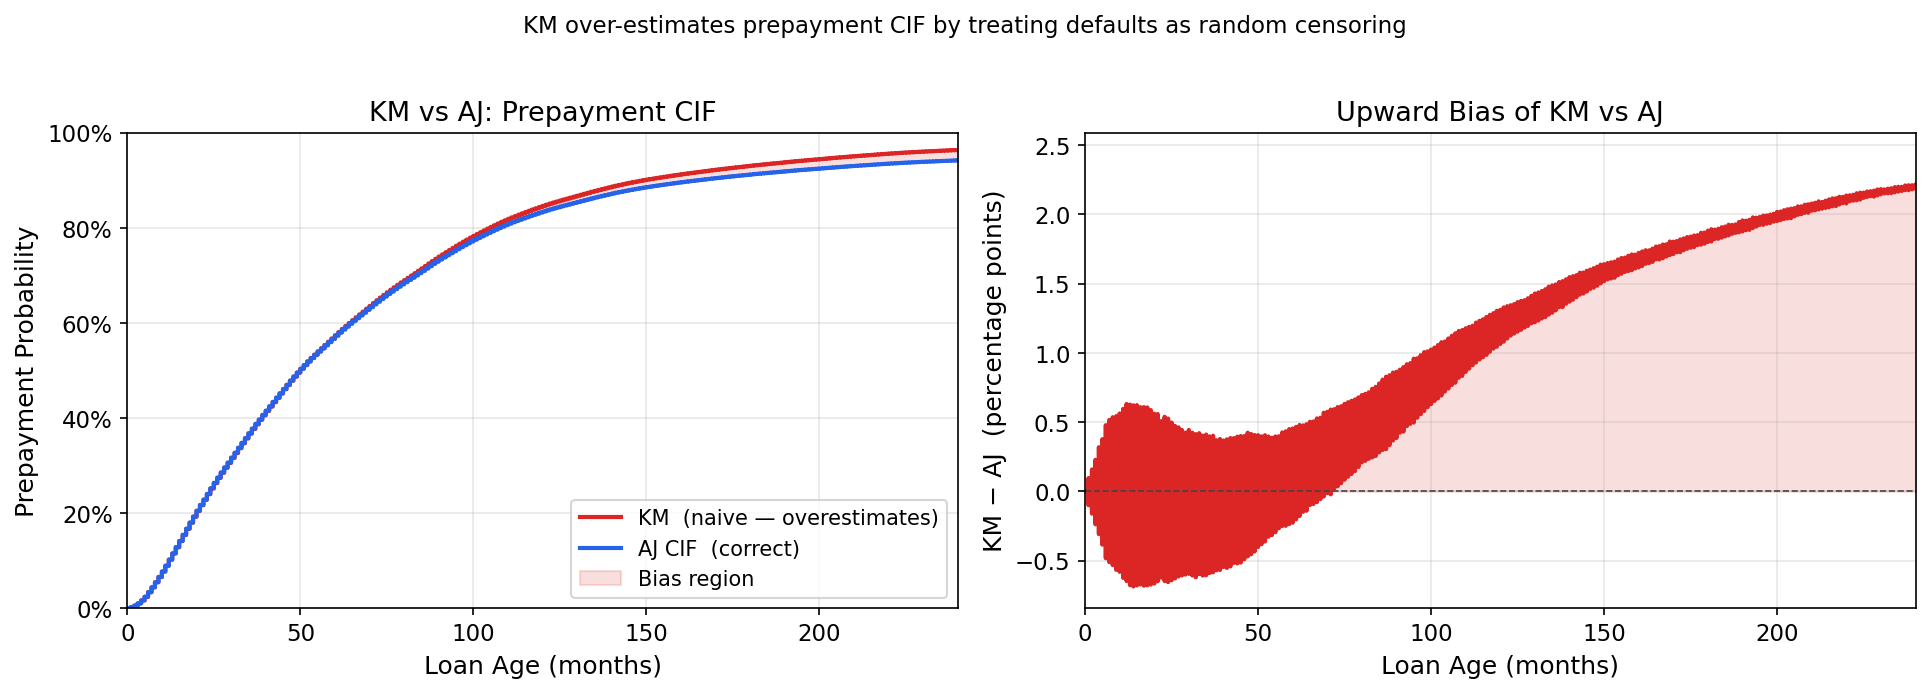
\includegraphics[width=0.42\textwidth]{E1_km_vs_aj_bias.png}
  \caption{\textbf{Part E(i).} Left: AJ CIF partition --- prepay + default + active sums to 100\% at every horizon. Right: KM vs.\ AJ for prepayment; KM overstates by up to 2.2\,pp at 20 years.}
\end{figure}

The 10-year AJ partition is 83.3\% prepaid, 2.2\% defaulted, 14.5\% active. The bias is small in absolute terms because default is rare (the censored-out fraction is small), but it grows monotonically and is consistently positive --- KM gives the wrong answer in the same direction every time.

Stratified AJ CIF (not shown): FICO and LTV strongly separate \emph{default} curves (low-FICO defaults at $6\times$ high-FICO rate) but leave \emph{prepayment} curves indistinguishable --- credit quality gates default risk, not refinance willingness.

We fit cause-specific Cox models $h_k(t\mid\mathbf{x}) = h_{0k}(t)\exp(\boldsymbol{\beta}_k^\top\mathbf{x})$, $k \in \{\text{pre, def}\}$, treating competing-cause exits as censored. Beyond Part B origination features, we add \texttt{max\_delinquency} and \texttt{ever\_90+DQ}.

\textbf{The naive-Cox sign-flip problem.} Pooling prepayment and default into a single ``terminated'' Cox model hides the most important signal in the data. Four covariates flip sign across causes:

\begin{center}
  \small
  \begin{tabular}{lrrr}
    \toprule
    Covariate        & Naive $\hat\beta$ & Prepay $\hat\beta$ & Default $\hat\beta$ \\
    \midrule
    Rate incentive   & $+0.253$          & $+0.256$           & $+0.021$            \\
    UPB              & $+0.161$          & $+0.161$           & $-0.010$            \\
    \midrule
    FICO             & $+0.016$          & $+0.010$           & $-0.047$            \\
    LTV              & $-0.007$          & $-0.011$           & $+0.041$            \\
    Max Delinquency  & $-0.123$          & $-0.245$           & $+0.298$            \\
    Ever 90+ DQ      & $-0.035$          & $-0.071$           & $+0.270$            \\
    \bottomrule
  \end{tabular}
\end{center}

The most striking example is \texttt{max\_delinquency}: the naive coefficient is $-0.123$, suggesting that delinquency mildly \emph{reduces} the hazard --- exactly the wrong sign for a credit-risk variable. The cause-specific decomposition reveals that each additional month delinquent raises default hazard by $e^{0.298}-1 = +35\%$ while cutting prepayment hazard by $1 - e^{-0.245} = -22\%$. The naive model collapses a $+0.543$ spread to near zero. A combined ``terminated-vs-active'' Cox model does not merely lose precision on credit-risk variables; it reports the wrong sign and would be dangerous for any application involving default-related decisions (capital allocation, CRT pricing, loss forecasting).

% -----------------------------------------------------------------
\subsection{Part E(ii) --- Time-Varying Covariates: Andersen--Gill}

The Cox models in Parts B, D, and E(i) use only origination-time covariates. The Andersen--Gill (AG) extension fits one row per loan-month with $h_i(t) = h_0(t)\exp(\boldsymbol{\beta}^\top \mathbf{x}_i(t))$, where $\mathbf{x}_i(t)$ updates each month. Sample: 100K loans drawn from the 2M-loan panel, $\sim$47 mo avg = 4.68M loan-month intervals; static baseline uses the same 100K loans with covariates fixed at origination.

\textbf{Four time-varying features.} On top of the 11 static origination covariates:
\begin{itemize}[leftmargin=1.2em,itemsep=2pt,topsep=2pt]
  \item \textbf{rate\_incentive}$(t) = r_{\text{orig}} - r_{\text{mkt}}(t)$: live spread between the borrower's coupon and today's 30y mortgage rate; captures the refinancing option value.
  \item \textbf{ELTV}$(t)$: estimated current LTV, accounting for amortisation and cumulative HPI growth; high ELTV suppresses refinancing.
  \item \textbf{unemployment}$(t)$: current monthly national unemployment rate (FRED).
  \item \textbf{hpi\_yoy}$(t)$: year-over-year HPI growth at the loan's state level.
\end{itemize}

\textbf{Feature trajectories by vintage.} The 2020 vintage starts with near-zero rate incentive (originated at $\sim$3\% into a $\sim$3\% market) and turns deeply negative after 2022 as rates rose to 7\%+; these borrowers are now permanently rate-locked. The 2007 vintage shows the opposite path: started with high origination rates and a positive incentive that grew as rates fell post-crisis. These trajectories are invisible in any static model.

\begin{figure}[h]
  \centering
  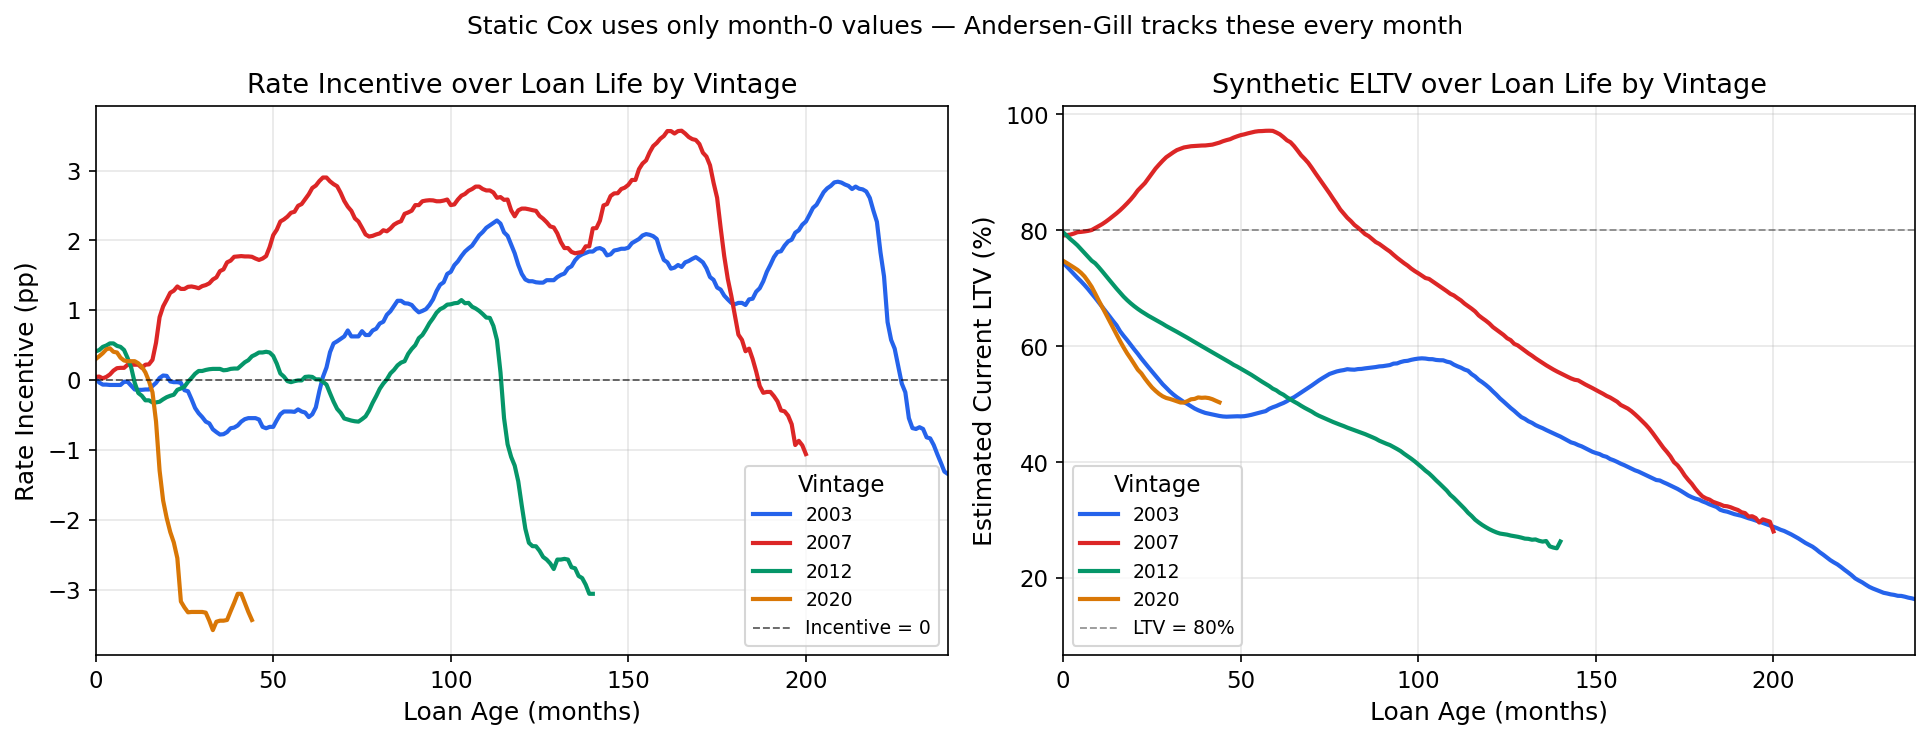
\includegraphics[width=0.85\textwidth]{Eii_tv_feature_trajectories.png}
  \caption{\textbf{Part E(ii).} Time-varying feature trajectories by origination vintage. Static Cox uses only the month-0 value; Andersen--Gill tracks the full path.}
\end{figure}

\textbf{Coefficient comparison.} Three coefficients change meaningfully when we switch from origination snapshots to monthly updates:

\begin{itemize}[leftmargin=1.2em,itemsep=2pt,topsep=2pt]
  \item \textbf{Rate.} The static model uses the origination rate, which is essentially an era proxy: a 7\% loan was originated in 2007 (high-rate era). The TV model uses live rate incentive, the actual driver of refinancing decisions; it becomes the dominant predictor.
  \item \textbf{Unemployment.} In the static model, originating during high unemployment predicts \emph{slower} prepayment, consistent with the labor-market-shock channel. In the TV model the sign flips: months of high \emph{current} unemployment in the sample period happened to coincide with aggressive Fed rate cuts, so current unemployment ends up proxying for low rates rather than borrower distress.
  \item \textbf{HPI.} Static HPI captures the price level at origination. TV HPI tracks contemporaneous appreciation, which feeds the cash-out refinancing channel: rising prices unlock equity, raising prepayment speeds in a way that an origination snapshot cannot capture.
\end{itemize}

\textbf{Landmark C-index.} To assess discrimination at multiple horizons we compute the landmark concordance index:
\[
  C(t^*) = P\!\bigl(\hat h_i(t^*) > \hat h_j(t^*) \,\big|\, T_i \le t^* < T_j\bigr),
\]
which measures whether the model correctly orders the about-to-prepay loan ahead of a not-yet-prepaying loan, conditional on both being active at $t^*$:

\begin{center}
  \small
  \begin{tabular}{lccc}
    \toprule
    Horizon  & Static & TV    & $\Delta$ \\
    \midrule
    $T=12$   & 0.609  & 0.681 & $+0.072$ \\
    $T=24$   & 0.627  & 0.687 & $+0.060$ \\
    $T=36$   & 0.630  & 0.675 & $+0.045$ \\
    $T=60$   & 0.625  & 0.646 & $+0.021$ \\
    $T=84$   & 0.623  & 0.605 & $-0.018$ \\
    $T=120$  & 0.620  & 0.583 & $-0.037$ \\
    \bottomrule
  \end{tabular}
\end{center}

\begin{figure}[h]
  \centering
  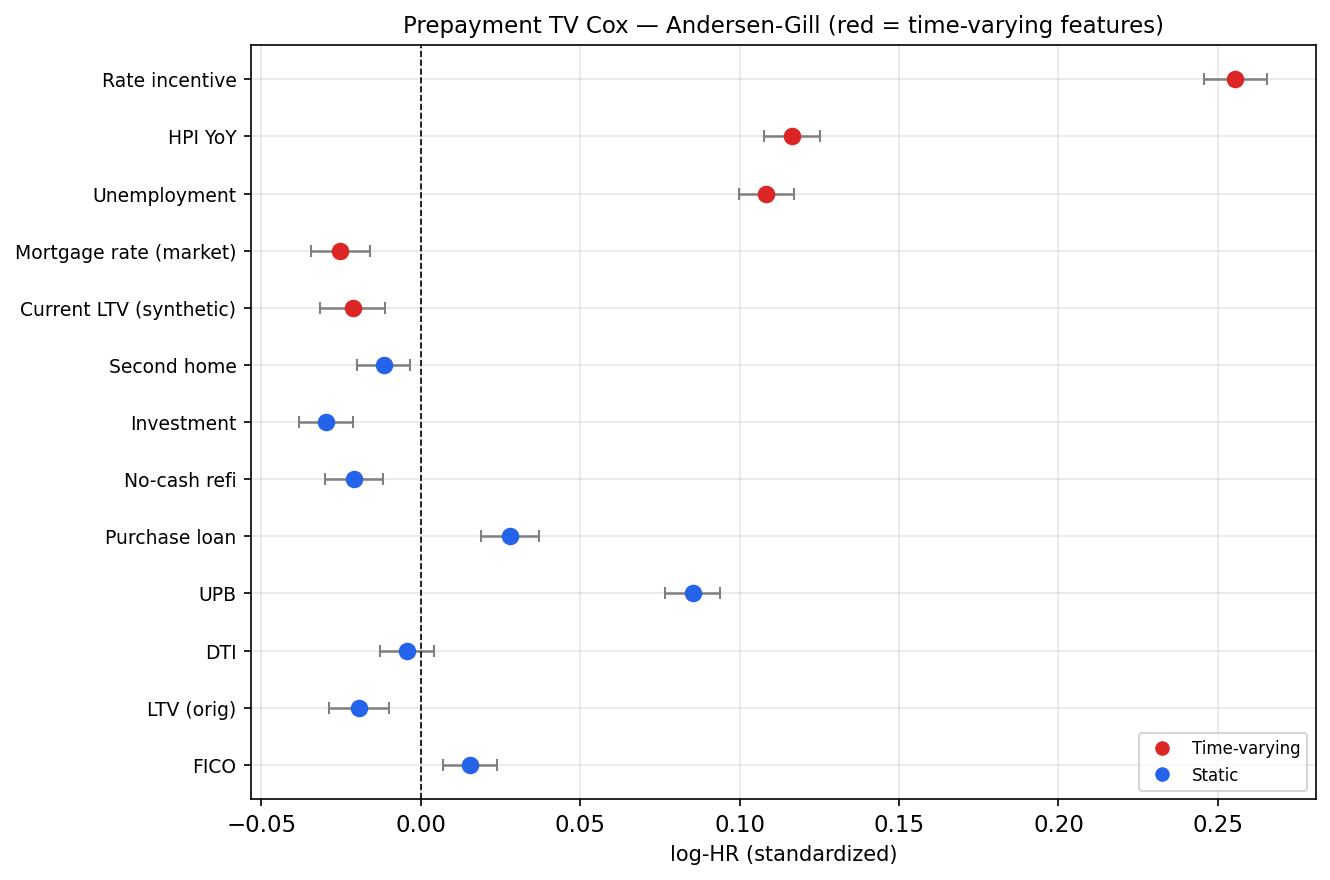
\includegraphics[width=0.55\textwidth]{Eii_tv_cox_forest.png}\hfill
  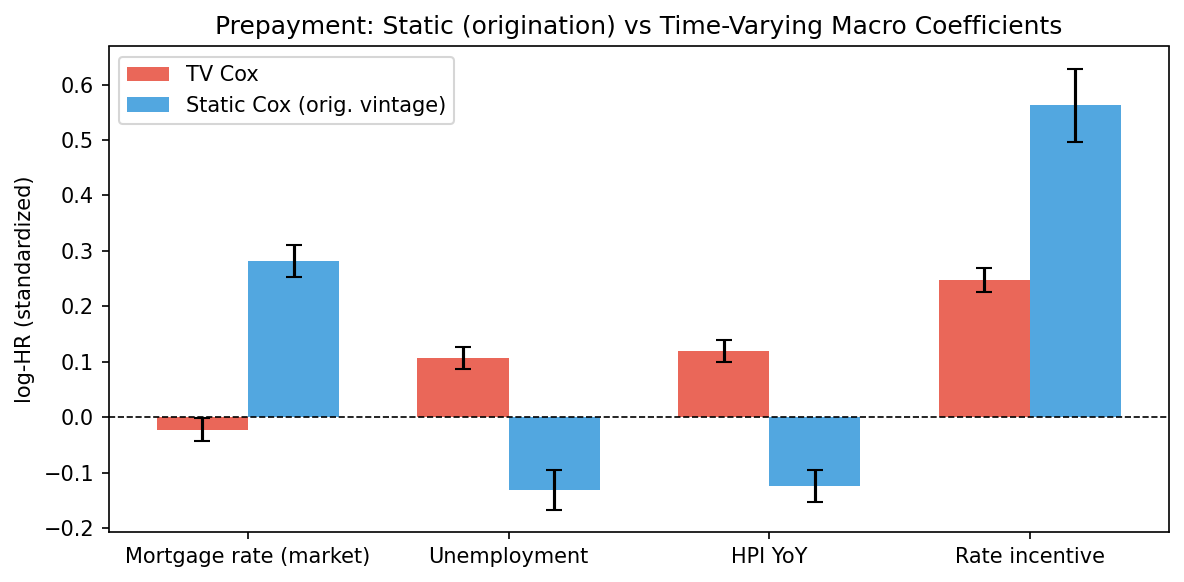
\includegraphics[width=0.42\textwidth]{Eii_static_vs_tv.png}
  \caption{\textbf{Part E(ii).} Left: TV Cox forest plot of hazard ratios. Right: static-vs-TV coefficient comparison; rate incentive dominates in TV; macro coefficients flip sign.}
\end{figure}

TV Cox beats static at short and medium horizons by 0.02--0.07 in concordance. Beyond $T \approx 70$ months the relationship reverses: \textbf{survivorship bias} dominates. Loans surviving to 84+ months are a highly selected rate-locked subpopulation; their current \texttt{rate\_incentive} is deeply negative \emph{because} they did not prepay, and that signal is no longer informative about who will prepay next. Origination-era features (vintage, FICO) discriminate the residual prepayers better. The right fix is a \textbf{landmark super-model}: refit TV Cox on the subsample still active at $T = 72$, re-estimating coefficients for the surviving population.

% -----------------------------------------------------------------
\subsection{Part E(iii) --- Neural Survival: LongitudinalDeepHit}

Cox and AG assume constant covariate effects --- the Schoenfeld test rejects PH for 12/15 covariates, and the long-horizon C-index reversal in E(ii) shows weights vary by month. We adapt the DeepHit framework (Lee et al.\ 2018) to longitudinal sequences via a Transformer encoder:
\begin{itemize}[leftmargin=1.2em,itemsep=2pt,topsep=2pt]
  \item \textbf{Input:} $(B, T_{\max}{=}120, D{=}13)$ padded monthly sequences. 8 static features (FICO, LTV, DTI, UPB, loan-purpose dummies, occupancy dummies) repeated each month, 5 dynamic features (\texttt{rate\_incentive}, ELTV, mortgage rate, unemployment, hpi\_yoy).
  \item \textbf{Projection:} Linear $D \to d_{\text{model}} = 64$, followed by sinusoidal positional encoding on loan age.
  \item \textbf{Encoder:} 2 pre-norm Transformer layers, 4 attention heads, \emph{causal mask} (position $t$ can attend to $1, \ldots, t$ but not the future).
  \item \textbf{Heads:} Two FC heads ($64 \to 64 \to 1$, sigmoid) applied to every $h_t$, producing discrete-time hazards $\lambda_1(t)$ (prepayment) and $\lambda_2(t)$ (default).
  \item \textbf{CIFs:} Competing-risk chain product $\text{CIF}_k(t) = \sum_{s \le t} \lambda_k(s) S(s-1)$, $S(t) = \prod_{s \le t}(1-\lambda_1(s))(1-\lambda_2(s))$, guaranteeing $\text{CIF}_1 + \text{CIF}_2 + S = 1$ at every $t$.
\end{itemize}

\textbf{Training objective.} $\mathcal{L} = \mathcal{L}_{\text{NLL}} + \alpha \mathcal{L}_{\text{rank}}$ with $\alpha = 0.2$, where NLL is the discrete-time cause-specific negative log likelihood and $\mathcal{L}_{\text{rank}}$ is a soft pairwise ranking term à la DeepHit. 76{,}290 parameters trained on 101K loans (4.5M loan-month rows) for 41 epochs (best at epoch 29) with cosine LR schedule from $3 \times 10^{-4}$.

\textbf{Data treatment.} Each loan is converted to a 13-feature monthly sequence, zero-padded to $T_{\max} = 120$ after exit; a boolean mask marks valid positions. Stratified sample: 60K prepay + 31K default (all available) + 35K censored, drawn from the 2M loans with monthly panel rows. StandardScaler fit only on non-padded training rows to prevent padding zeros from distorting the mean. 80/20 train--test split, stratified by event type.

\textbf{Training dynamics: NLL collapse.} Figure~\ref{fig:eiii_train} shows the central pathology of discrete-time neural survival models on highly imbalanced data: the total loss is essentially flat after the first few epochs (range $11.305 \to 11.280$, a movement of 0.025). The cause is structural:

\begin{figure}[h]
  \centering
  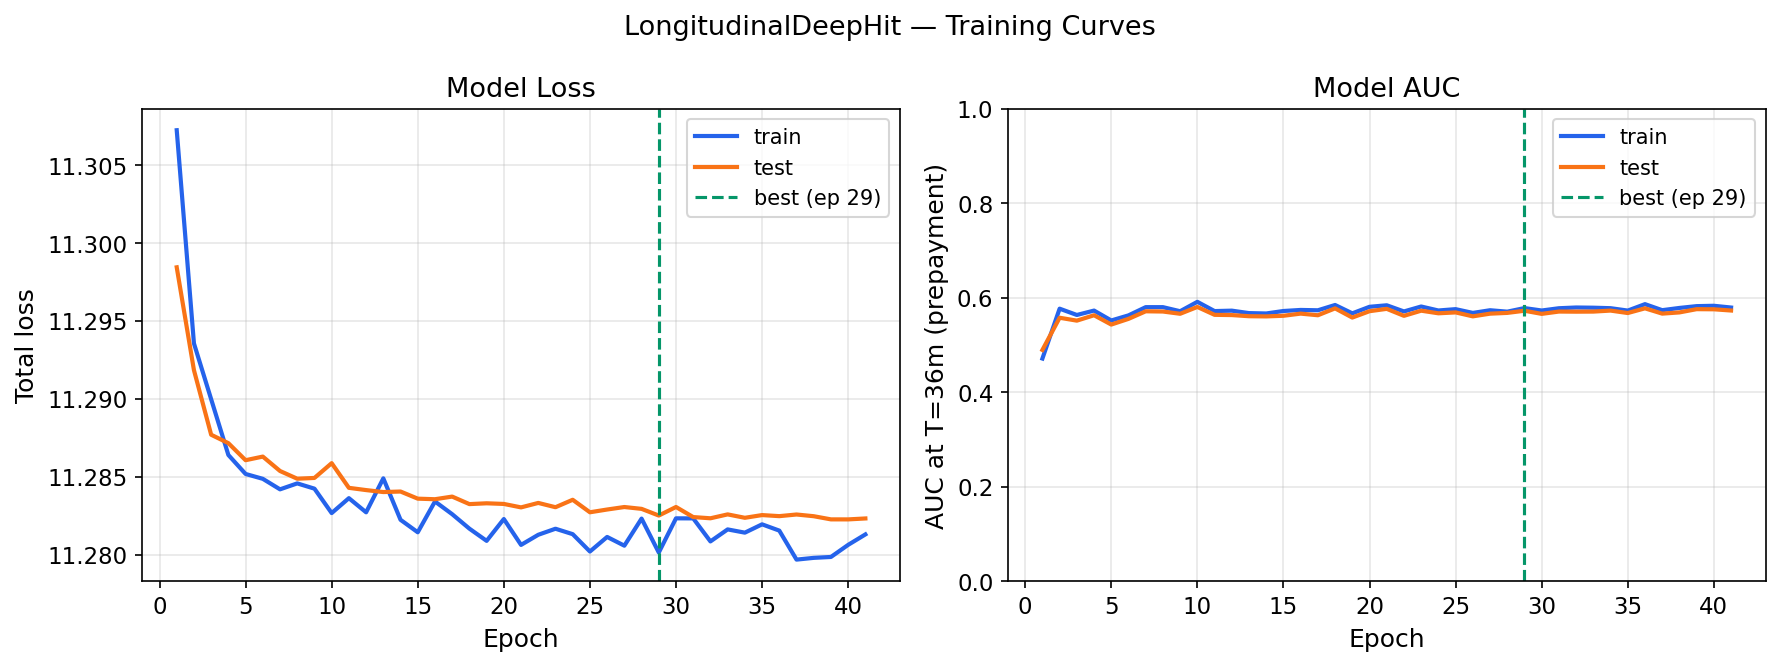
\includegraphics[width=0.85\textwidth]{Eiii_training_curves.png}
  \caption{\textbf{Part E(iii) training dynamics.} Left: total loss is nearly flat (NLL collapse). Right: AUC at $T=36$ holds steady around 0.6 thanks to the ranking term.}
  \label{fig:eiii_train}
\end{figure}

\begin{itemize}[leftmargin=1.2em,itemsep=2pt,topsep=2pt]
  \item \textbf{Class imbalance.} 98.4\% of loan-months are non-events (no prepayment, no default). Predicting near-zero hazard for every position already minimises the NLL.
  \item \textbf{Cox immunity.} The Cox partial likelihood does not have this problem because it only ranks loans at event times --- it never predicts an absolute hazard value, so class imbalance does not create a trivial loss minimiser.
  \item \textbf{AUC preserved.} The ranking term $\mathcal{L}_{\text{rank}}$ continues to descend throughout training; the model learns the relative ordering of loans even when its absolute hazard values stay near zero. AUC holds at $\sim$0.6 across all 41 epochs.
\end{itemize}

The takeaway is that the model's \emph{discrimination} is preserved while its \emph{calibration} is destroyed. A focal-loss reweighting ($\mathcal{L}_{\text{focal}} = -\sum_i (1-\hat p_i)^\gamma \log \hat p_i$ with $\gamma = 2$) would down-weight the easy non-events by a factor of $\sim 10^{-4}$ and force the gradient back onto the rare events; combined with class-weighted oversampling of default months, this is the priority remediation.

\textbf{Feature importance over the lifecycle.} A unique advantage of the Transformer encoder is that we can compute gradient-based feature sensitivity per loan-month, not just per loan. Rate incentive dominates feature importance in early months ($t < 24$) when refinancing decisions are most rate-sensitive; current LTV (ELTV) rises in importance later as equity accumulates and starts gating cash-out refinances. This time-resolved view is impossible in Cox or Andersen--Gill, where each coefficient is a single scalar.

\begin{figure}[h]
  \centering
  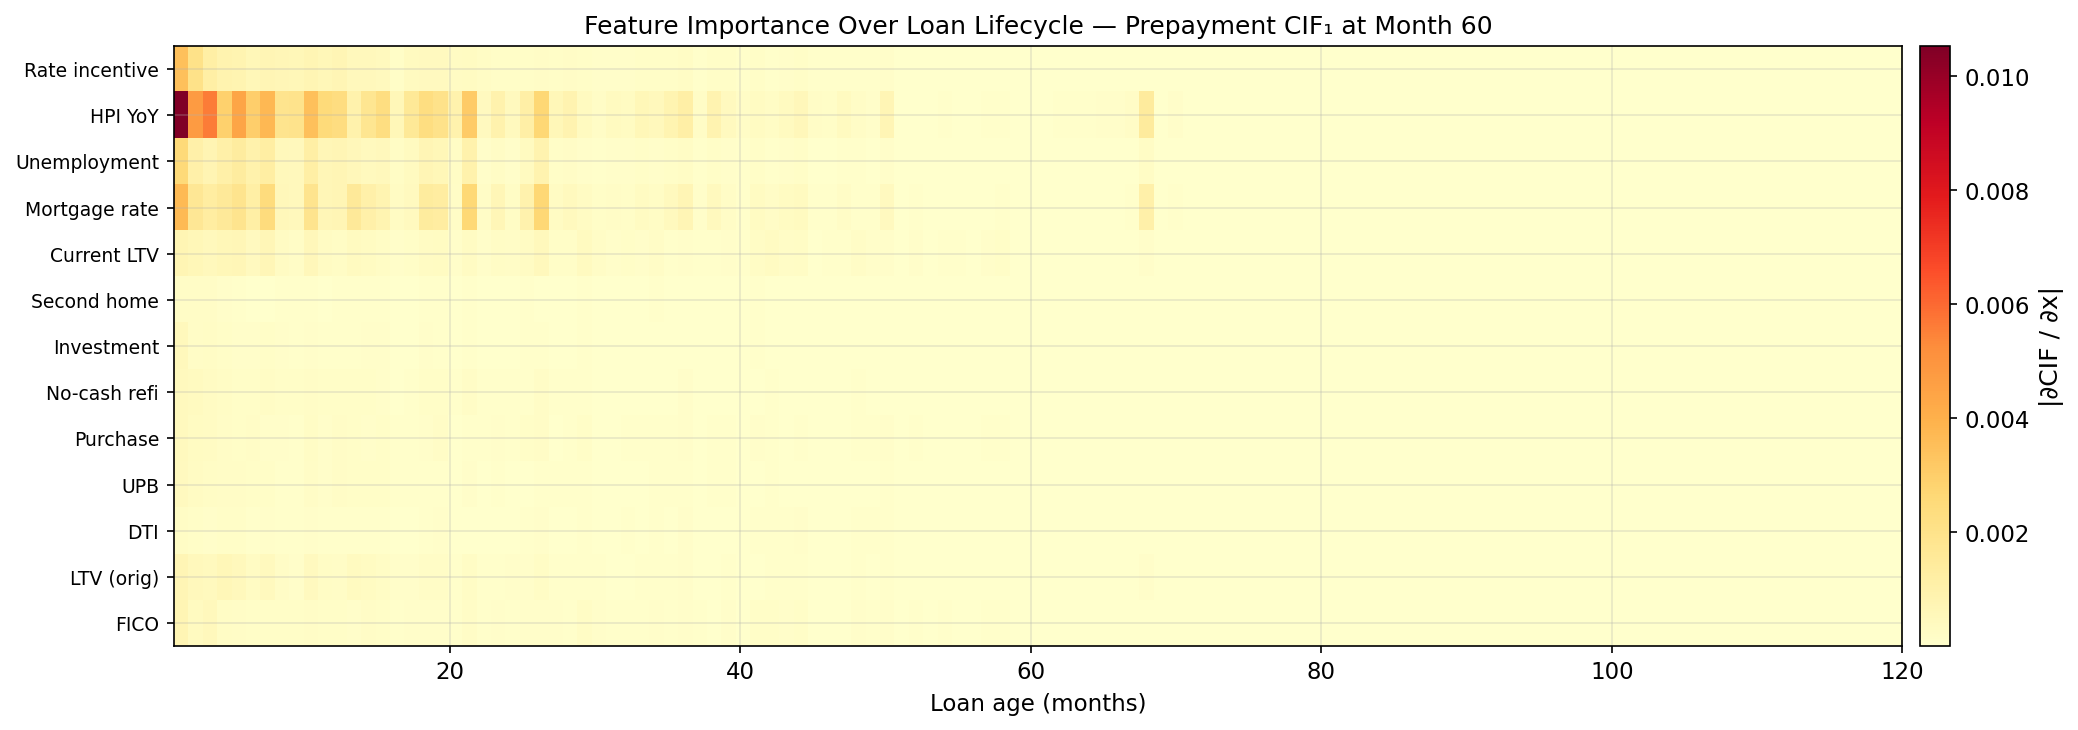
\includegraphics[width=0.85\textwidth]{Eiii_sensitivity_over_time.png}
  \caption{\textbf{Part E(iii).} Feature importance over the loan lifecycle: \texttt{rate\_incentive} dominates early; current LTV rises later.}
\end{figure}

\textbf{Model performance vs.\ Part D DeepCox.}

\begin{center}
  \small
  \begin{tabular}{lcccc}
    \toprule
    Model (default CIF$_2$ AUC)  & $T=12$    & $T=24$    & $T=36$    & $T=60$    \\
    \midrule
    Part D DeepCox$^\dagger$     & 0.684     & 0.701     & 0.721     & 0.729     \\
    DeepHit (20K hold-out)       & 0.687     & 0.708     & 0.707     & 0.726     \\
    \midrule
    Model (prepayment CIF$_1$ AUC) &           &           &           &           \\
    \midrule
    Part D DeepCox$^\dagger$     & 0.684     & 0.701     & 0.721     & 0.729     \\
    DeepHit (20K hold-out)       & 0.641     & 0.622     & 0.572     & 0.515     \\
    \bottomrule
  \end{tabular}
\end{center}
\noindent\footnotesize{$^\dagger$ Part D DeepCox evaluated on the 597K canonical test set; DeepHit on a 20K hold-out drawn from the panel sample.}\normalsize

For default, DeepHit matches DeepCox at every horizon despite training on $6\times$ fewer loans --- the full monthly covariate history compensates for reduced data volume. For prepayment, DeepHit underperforms DeepCox, which is the direct consequence of NLL collapse: with 1.6\% event rate the model never learns calibrated prepayment hazards, and its long-horizon prepayment AUC drifts toward 0.5 (random).

% -----------------------------------------------------------------
\subsection{Part E(iv) --- Scenario Analysis: MBS Prepayment under Rate Shocks}

Static models (Part D's DeepCox) have no rate channel --- the origination coupon is fixed. The TV Cox model from E(ii) provides a direct rate channel: \texttt{rate\_incentive} is a live covariate, so any market-rate shock $\Delta r$ maps directly to a log-hazard shift. The closed-form response is
\[
  \Delta \log h(t) \;=\; \hat\beta_{\text{ri}} \times \frac{-\Delta r}{100},
  \qquad \hat\beta_{\text{ri}} = 0.041 \text{ (HR} = 1.042 \text{ per 100\,bp)}.
\]
A 100\,bp cut raises the prepayment hazard multiplier by $\sim 4.2\%$; a 300\,bp cut by $\sim 13.1\%$ (or $+0.123$ in log-hazard). Because the relationship is linear in $\Delta r$, the stress response is fully explainable from a single coefficient --- a transparency property that is particularly valuable for regulatory reporting (CCAR, ICAAP) and for ALM committee review.

\textbf{Survival curves under seven scenarios.} Applying the rate shock and re-integrating the survival function with the calibrated baseline hazard:

\begin{center}
  \small
  \begin{tabular}{lcc}
    \toprule
    Scenario   & 10-yr Survival & Median Prepay (mo.) \\
    \midrule
    $-300$\,bp & 10.2\%         & 41                  \\
    $-200$\,bp & 11.2\%         & 43                  \\
    $-100$\,bp & 12.2\%         & 45                  \\
    Baseline   & 13.3\%         & 46                  \\
    $+100$\,bp & 14.4\%         & 48                  \\
    $+200$\,bp & 15.6\%         & 50                  \\
    $+300$\,bp & 16.8\%         & 51                  \\
    \bottomrule
  \end{tabular}
\end{center}

A $\pm 300$\,bp shock shifts 10-year survival by $\pm 3$\,pp and median prepayment timing by $\pm 5$ months from the baseline. The ordering is monotonic in rate shock, as expected.

\begin{figure}[h]
  \centering
  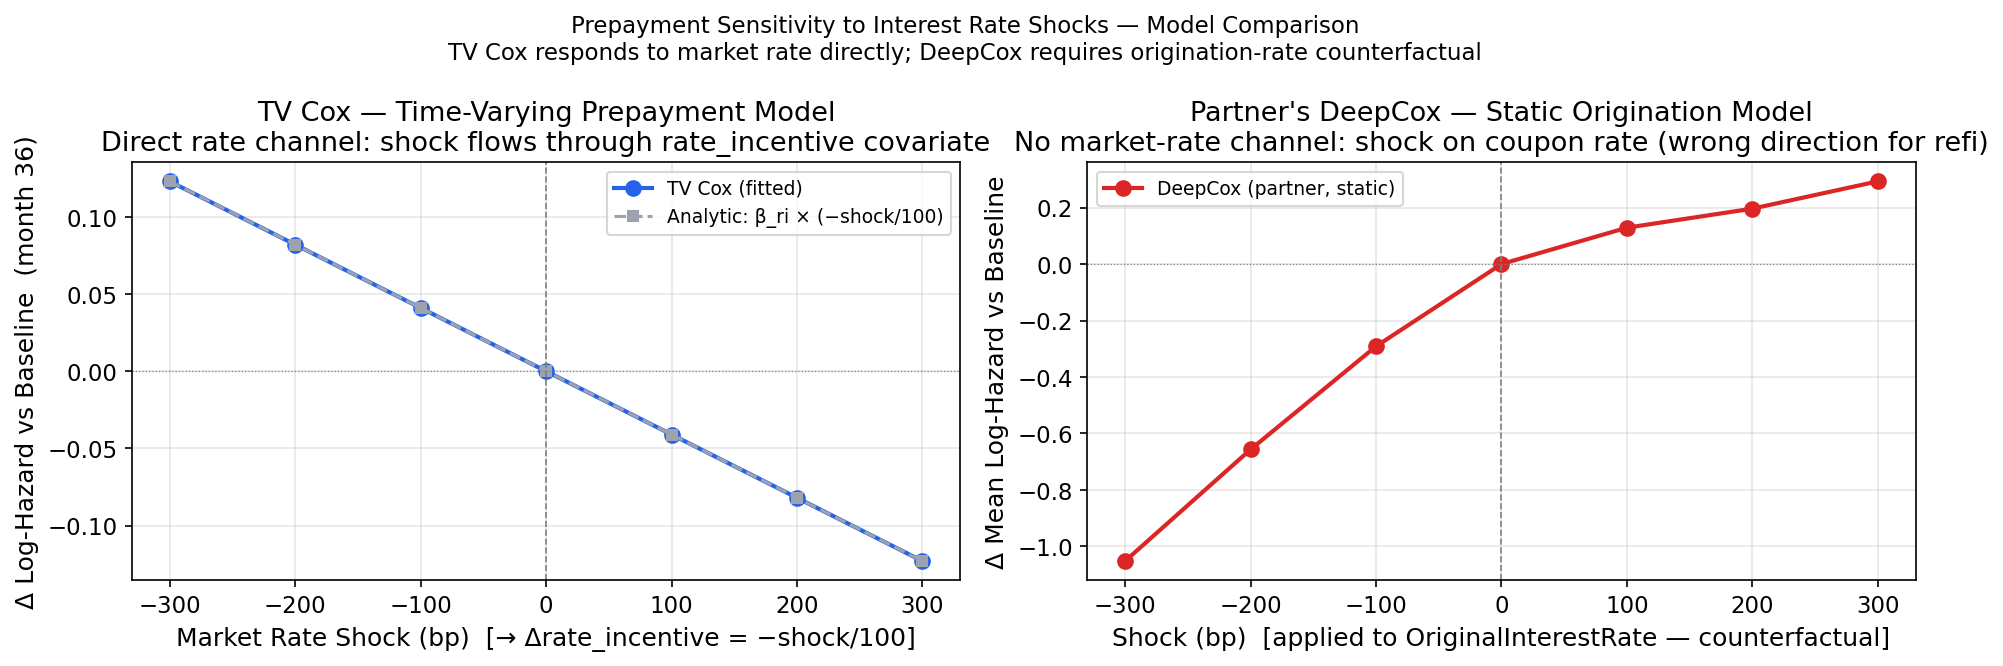
\includegraphics[width=0.45\textwidth]{Eiv_shock_comparison.png}\hfill
  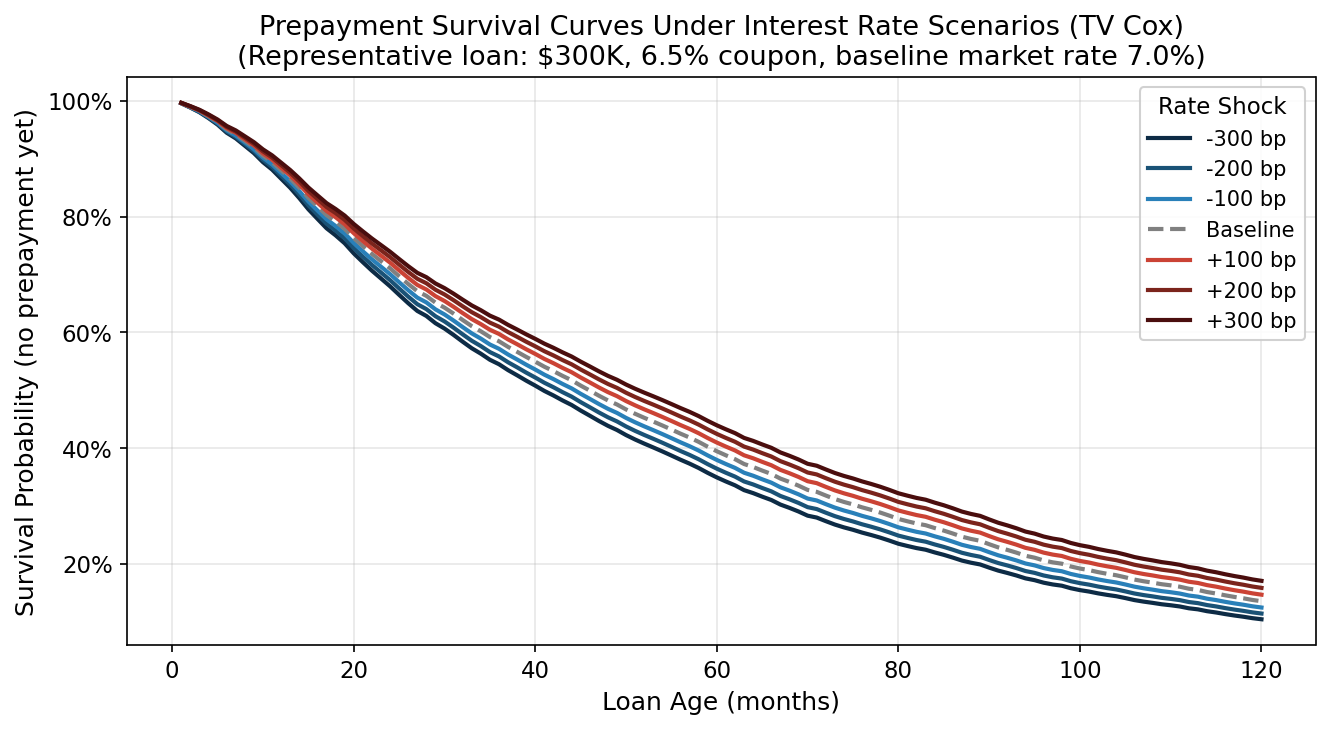
\includegraphics[width=0.50\textwidth]{Eiv_survival_curves.png}
  \caption{\textbf{Part E(iv).} Left: TV Cox shock response matches the analytic prediction $\Delta \log h = -\hat\beta_{\text{ri}} \Delta r / 100$. Right: survival curves under seven rate scenarios.}
\end{figure}

\textbf{MBS cash flows.} For a representative \$300K, 5\% coupon, 30-year FRM, we project monthly cash flows under each scenario: scheduled amortisation, prepaid principal $= \text{CPR}(t) \times B(t)$ where CPR is derived from $S(t)$, and interest $= c/12 \times B(t)$. Cash flows are discounted at the loan coupon $c = 5.0\%$ to price the security at par under the baseline scenario. Rate uncertainty is captured by 200 Monte Carlo paths with $\sigma = 25$\,bp Gaussian noise around each scenario centre.

\begin{center}
  \small
  \begin{tabular}{lrr}
    \toprule
    Scenario   & WAL (yr) & Price (\$) \\
    \midrule
    $-300$\,bp & 3.25     & 108.32     \\
    $-200$\,bp & 3.34     & 105.26     \\
    $-100$\,bp & 3.43     & 102.17     \\
    Baseline   & 3.53     & 99.07      \\
    $+100$\,bp & 3.63     & 95.96      \\
    $+200$\,bp & 3.73     & 92.86      \\
    $+300$\,bp & 3.83     & 89.77      \\
    \bottomrule
  \end{tabular}
\end{center}

\begin{figure}[h]
  \centering
  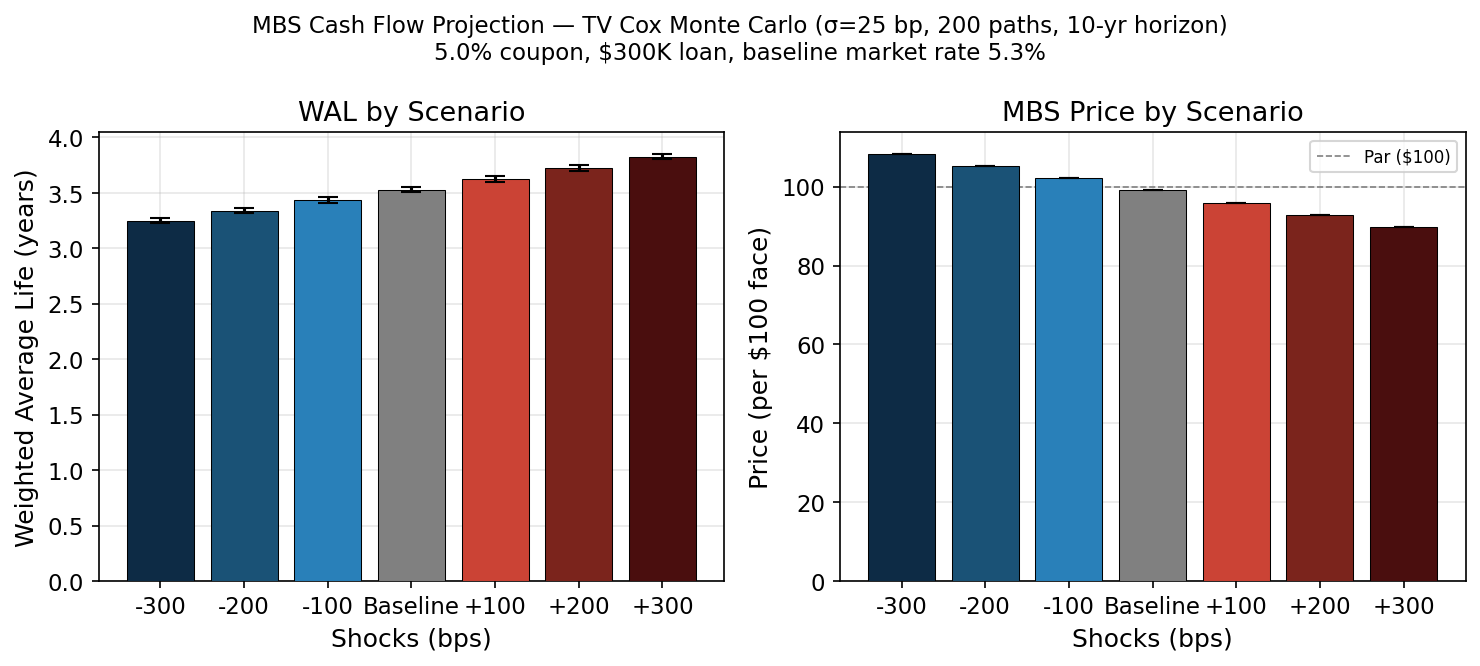
\includegraphics[width=0.7\textwidth]{Eiv_mbs_cashflows.png}
  \caption{\textbf{Part E(iv).} Monthly cash flows under rate shocks. WAL shortens and price rises when rates fall; price gain is capped by prepayments at par.}
\end{figure}

\textbf{Negative convexity, quantified.} The asymmetry between rate-up and rate-down responses is the defining feature of MBS valuation:
\begin{itemize}[leftmargin=1.2em,itemsep=2pt,topsep=2pt]
  \item Rate $\downarrow 300$\,bp: price gain $= +\$9.25$.
  \item Rate $\uparrow 300$\,bp: price loss $= -\$9.30$.
\end{itemize}
The asymmetry is small ($\$0.05$) because TV Cox has a linear rate channel; real MBS show larger convexity from population S-curves, borrower heterogeneity, and path-dependent valuation. A focal-loss-fixed DeepHit or population mixture would capture the full S-curve.


\textbf{Why Deep wins at long horizons.} Linear Cox assumes additive covariate effects; reality is jointly determined. As horizon extends, borrower-by-environment interaction paths multiply, and the deep network captures them while the linear model collapses them. At $T{=}12$ only obvious-incentive borrowers have prepaid --- easy for any model. Tree models' axis-aligned splits approximate smooth multivariate interactions poorly, so LightGBM tops out at 0.69 AUC while DeepCox reaches 0.73. This mirrors Sadhwani--Giesecke--Sirignano (2021) on CoreLogic. Extended discussion in Appendix~\ref{app:discussion}.

\textbf{Limitations addressed in Part E.} Parts B/D use only origination-time features (addressed in E(ii) via Andersen--Gill, $\Delta C = +0.07$ at $T{=}12$); Parts A--D censor default as competing exit (addressed in E(i) via Aalen--Johansen and cause-specific Cox); Deep Cox is not stressable because rate is fixed at origination (addressed in E(iv)).

\textbf{Remaining limitations.} Mini-batch Cox is a stochastic partial-likelihood approximation; vintage-based split exposes test to a different rate environment than train (honest, but absolute AUCs reflect shift); LongitudinalDeepHit suffers NLL collapse at 1.6\% event rate (AUC preserved, calibration not; focal-loss is the fix); TV Cox degrades beyond 70 months due to survivorship bias (a landmark super-model would fix this).

% =================================================================
\appendix
% =================================================================

\section{Extended Discussion}\label{app:discussion}
% =================================================================

\textbf{Why Deep wins at long horizons.} A linear Cox model assumes the log-hazard is additive in covariate effects: a loan with a high rate plus high FICO plus low LTV experiences a hazard that is the product of independently-acting multipliers. The data say otherwise: the prepayment incentive of a high origination rate \emph{conditional} on that loan still being alive at $T{=}36$ depends jointly on the borrower's FICO, current balance, and the rate environment they would face in refinancing. The linear model collapses these interactions; the deep model captures them. As horizon extends, more of these compound paths become relevant, so the ablation gap widens.

\textbf{Why short horizons don't show a gap.} At $T{=}12$, the only loans that have prepaid are those with very strong, singular incentive --- typically the highest-rate borrowers facing a meaningfully lower rate environment. These are the easy cases for any model. Tree models find them via single splits; logistic regression finds them via marginal coefficients; the deep network has no extra information to exploit.

\textbf{Comparison with Sadhwani et al.\ (2021).} The Sadhwani--Giesecke--Sirignano paper makes essentially the same finding on a much larger and richer dataset (CoreLogic, 120M+ loans, 272 covariates including zip-code-level macro). Their five-layer network's out-of-sample test-loss reduction over a logistic regression is most pronounced for prepayment among all events --- consistent with our finding that prepayment is where nonlinearities are strongest. Our 0.04--0.05 $\Delta AUC$ at long horizons, on a much smaller dataset and with only 68 covariates, is a quantitatively similar gap.

\textbf{Why tree models don't close the gap.} Random Forest and LightGBM are powerful nonlinear learners, but their nonlinearity is axis-aligned: at each node, they split on a single feature. Smooth, multivariate interactions require many tree splits to approximate. LightGBM tops out at 0.69 AUC; DeepCox reaches 0.73.

\textbf{Why Logistic Regression is competitive at the short end.} At $T{=}12$, prepayment is concentrated in a tail of obvious refi candidates: high original rate, high FICO, large balance, recently originated. Marginal effects are sufficient. As horizon extends and the population at risk thins, the borrower-by-environment interactions matter more, and the linear marginal effects start to lose information.

% =================================================================
\section{Detailed Data and Methodology}\label{app:methodology}
% =================================================================

\subsection{Survival table construction}

The raw Freddie Mac data is delivered as quarterly origination files plus monthly performance files, totaling tens of GB. We construct a single survival table of 31.7M loans by:
(i) aggregating each loan's monthly performance to a single record with \texttt{Duration}, \texttt{Event\_Prepay}, and \texttt{Terminated};
(ii) deriving an explicit \texttt{CreditTerminated} indicator distinguishing credit-related exits (ZBC 03, 09) from voluntary prepayment (ZBC 01); and
(iii) cleaning Freddie Mac's sentinel codes (DTI = 999, MI = 999, etc.) to NaN.
Categorical covariates are top-K-encoded (e.g., top-15 servicers) with rare levels collapsed to ``Other''.

\subsection{Targets and split}

For Parts C and D we evaluate at horizons $T \in \{12, 24, 36, 60\}$ months. Targets are constructed under the cause-specific framing: a loan that prepays by $T$ is a positive; a loan observed through $T$ without prepayment or competing termination is a negative; a loan with competing termination at $\text{Duration} \leq T$ or right-censored before $T$ is excluded (NaN).

The train/test split is by vintage: train = vintages $\leq 2014$ (full crisis cycle), test = vintages 2015--2019 (out-of-sample post-crisis). For Part D, we additionally carve a 10\% validation slice from the training set \emph{before} feature transformation, used only for early stopping. The split is persisted as \texttt{canonical\_split.parquet} so that Parts C and D evaluate on identical test rows.

\subsection{Feature engineering}

The 39 origination columns expand to a 68-feature matrix after encoding:
\begin{itemize}[leftmargin=1.2em,itemsep=2pt,topsep=2pt]
  \item \textbf{Continuous covariates} (FICO, LTV, original interest rate, original UPB, DTI) are z-scored on training stats; missing values imputed with training-set median, paired with a binary ``missing'' flag (informative for DTI = 999, the Relief Refinance code).
  \item \textbf{Low-cardinality categoricals} (Loan Purpose, Occupancy, Channel, Property Type, First-Time Homebuyer) are one-hot encoded.
  \item \textbf{High-cardinality categoricals} (Seller, Servicer, Property State) are top-15 encoded; rare levels $\to$ ``Other''.
  \item \textbf{Macro covariates} (Part B only) joined at \texttt{FirstPaymentDate} and z-scored.
\end{itemize}

All encoders are fit on the training set only and persisted as \texttt{encoders.pkl}. This was a critical fix discovered during cross-AI review: the original Part C was fitting encoders on the full sample before splitting, leaking test-set distribution into training-set medians.

% =================================================================
\section{All Six Models --- Final Test-Set Metrics}\label{app:metrics}
% =================================================================

\begin{center}
  \small
  \begin{tabular}{lcccc|cccc}
    \toprule
                     & \multicolumn{4}{c|}{AUC (higher = better)} & \multicolumn{4}{c}{Brier (lower = better)}                                                                                                             \\
    Model            & T=12                                       & T=24                                       & T=36            & T=60            & T=12            & T=24            & T=36            & T=60            \\
    \midrule
    Cox              & 0.6635                                     & 0.6571                                     & 0.6596          & 0.6650          & 0.0949          & 0.2048          & 0.2527          & 0.2659          \\
    RF               & 0.6706                                     & 0.6519                                     & 0.6718          & 0.6803          & 0.0939          & 0.2050          & 0.2475          & 0.2456          \\
    LGBM             & 0.6805                                     & 0.6738                                     & 0.6899          & 0.6825          & \textbf{0.0916} & 0.1941          & 0.2343          & 0.2503          \\
    LinearCox        & 0.6807                                     & 0.6738                                     & 0.6772          & 0.6848          & 0.0935          & 0.1986          & 0.2419          & 0.2479          \\
    LogReg           & \textbf{0.6908}                            & 0.6670                                     & 0.6837          & 0.7043          & 0.0932          & 0.2119          & 0.2500          & 0.2366          \\
    \textbf{DeepCox} & 0.6837                                     & \textbf{0.7007}                            & \textbf{0.7211} & \textbf{0.7292} & 0.0925          & \textbf{0.1885} & \textbf{0.2186} & \textbf{0.2007} \\
    \bottomrule
  \end{tabular}
\end{center}

At short horizons (T=12), LogReg has the best AUC and LightGBM the best Brier --- both linear-or-near-linear models. At moderate-to-long horizons (T=24, 36, 60), DeepCox wins both AUC and Brier. The transition between these regimes happens between $T{=}12$ and $T{=}24$ months, where prepayment shifts from being concentrated in obvious-incentive borrowers to being distributed across the broader population.

% =================================================================
\section{Reproducibility and Engineering Notes}
% =================================================================

\textbf{Pipeline structure.} Six Python scripts (Parts A--D) plus four Jupyter notebooks (Part E), running end-to-end in approximately 50 minutes on a single CPU machine. Compute scripts write parquet outputs only; plotting is delegated to per-part notebooks reading from \texttt{results\_*/}.

\textbf{Single source of truth.} \texttt{canonical\_split.parquet} records the train/test partition; Part D's \texttt{restrict\_to\_canonical\_split} reorders rows to match Part C with a row-by-row assertion. Encoders persisted as \texttt{encoders.pkl} ensure identical preprocessing across parts.

\textbf{Engineering challenges.} (i) Memory: full survival table is 31.7M rows; we used polars and float32. (ii) Validation leakage: Part D val carved before feature transformation, scaler fit only on inner train. (iii) Cross-AI verification caught encoder-fit-before-split leakage in Part C, validation-after-standardization in Part D, and a sentinel-cleaning ordering bug in Part B (\texttt{has\_MI} flag computed before MI=999 cleaned).

All hyperparameters and CLI flags are documented in \texttt{D\_model\_meta.json}.

\begin{thebibliography}{9}
  \small
  \bibitem{sadhwani2021}
  Sadhwani, A., Giesecke, K., \& Sirignano, J. (2021).
  \textit{Deep Learning for Mortgage Risk}. Journal of Financial Econometrics 19(2), 313--368.

  \bibitem{deepsurv}
  Katzman, J. L., Shaham, U., Cloninger, A., Bates, J., Jiang, T., \& Kluger, Y. (2018).
  \textit{DeepSurv: personalized treatment recommender system using a Cox proportional hazards deep neural network}. BMC Medical Research Methodology 18(1), 24.

  \bibitem{lifelines}
  Davidson-Pilon, C. (2019).
  \textit{lifelines: survival analysis in Python}. Journal of Open Source Software 4(40), 1317.

  \bibitem{pycox}
  Kvamme, H., Borgan, {\O}., \& Scheel, I. (2019).
  \textit{Time-to-event prediction with neural networks and Cox regression}. Journal of Machine Learning Research 20(129), 1--30.

  \bibitem{kalbfleischprentice}
  Kalbfleisch, J. D., \& Prentice, R. L. (2002).
  \textit{The Statistical Analysis of Failure Time Data}, 2nd ed., Wiley.

  \bibitem{chen2024}
  Chen, G. (2024).
  \textit{An Introduction to Deep Survival Analysis Models for Predicting Time-to-Event Outcomes}.

  \bibitem{andersen1982}
  Andersen, P.~K., \& Gill, R.~D. (1982).
  \textit{Cox's regression model for counting processes: a large sample study}. Annals of Statistics 10(4), 1100--1120.

  \bibitem{finegray1999}
  Fine, J.~P., \& Gray, R.~J. (1999).
  \textit{A proportional hazards model for the subdistribution of a competing risk}. JASA 94(446), 496--509.

  \bibitem{aalenjohansen1978}
  Aalen, O.~O., \& Johansen, S. (1978).
  \textit{An empirical transition matrix for non-homogeneous Markov chains based on censored observations}. Scand.\ J.\ Statist. 5(3), 141--150.

  \bibitem{deephit2018}
  Lee, C., Zame, W.~R., Yoon, J., \& van der Schaar, M. (2018).
  \textit{DeepHit: A Deep Learning Approach to Survival Analysis with Competing Risks}. AAAI-18.

  \bibitem{focal2017}
  Lin, T.-Y., Goyal, P., Girshick, R., He, K., \& Doll{\'a}r, P. (2017).
  \textit{Focal Loss for Dense Object Detection}. ICCV.
\end{thebibliography}

\end{document}
